%!TEX root = ../main.tex
% \documentclass[a4paper,12pt]{article}
% \usepackage[english]{babel} % (pjl) Need to uncomment this later.
% \usepackage{enumerate}
% \usepackage{hyperref}
% \usepackage{amsmath,amsfonts,amsthm}
% \usepackage{tikz}%\usepackage{mathrsfs,color}
% %\usepackage[colorlinks=true]{hyperref}
% \allowdisplaybreaks
% \usepackage{mathtools}
% \usepackage{pdfsync} % (pjl) Need to uncomment this later.
% \usepackage{graphicx,float}
% \usepackage{mathrsfs} % For script 'L' Laplace transform font.
% \usepackage{array} % Improves `tabular` and `array` environments
% %   \usepackage{slashbox} % Defines \backslashbox{..}{..}                                                % need for `show only references'
% %\mathtoolsset{showonlyrefs=true}                                    % only equations which are labeled AND referenced will be numbered.

% \usepackage[utf8]{inputenc}
% \usepackage{authblk}
% \usepackage[T1]{fontenc}
% \usepackage{lmodern}

% \usepackage{color}
% \newtheorem{lemma}{Lemma}
% \newtheorem{theo}{Theorem}
% \newtheorem{corollary}{corollary}
% \newtheorem{proposition}{proposition}
% \newtheorem{remark}{remark}[section]
% \newtheorem{example}{example}

% \newtheorem{definition}{definition}
% \newtheorem{hp}{Assumption}
% \textwidth=16cm
% \textheight=24cm
% \setlength{\topmargin}{-.8in}
% \setlength{\oddsidemargin}{0.0in}

% % To delete
% \newcommand{\Lap}{\mathscr{L}}
% \newcommand{\G}{\mathcal{G}} % Probability generating function

% \renewcommand{\baselinestretch}{1}

% \newcommand{\e}{\mathrm{e}} % 2.71..
% \newcommand{\E}{\mathbb{E}} % Expected value
% \newcommand{\Esp}[1]{\Esp\left(#1\right)} %..?
% \renewcommand{\P}{\mathbb{P}} % Probability
% % \renewcommand{\Pr}[1]{\P\left(#1\right)} % Probability
% \newcommand{\C}{\mathbb{C}} % Complex numbers
% \newcommand{\R}{\mathbb{R}} % Real numbers
% \newcommand{\N}{\mathbb{N}_0} % Natural numbers
% \newcommand{\Npos}{\mathbb{N}_+} % Natural numbers
% \newcommand{\Z}{\mathbb{Z}} % Integers
% \newcommand{\Lp}{L} % L-p spaces
% \newcommand{\PGF}{\mathcal{G}} % Probability generating function
% \newcommand{\LT}[1]{\mathcal{L}\{#1\}} % Laplace transform
% \newcommand{\LTsub}[1]{\mathcal{L}_{#1}} % Laplace transform subscript
% % \newcommand{\FT}[1]{\mathcal{F}\{#1\}} % Fourier transform
% % \newcommand{\FTsub}[1]{\mathcal{F}_{#1}} % Fourier transform subscript
% \newcommand{\Ind}{\mathbb{I}} % Indicator

% \newcommand{\dd}{\,\mathrm{d}} % dx etc
% \newcommand{\ddd}{\mathrm{d}} % F(dz) etc
% \newcommand{\ih}{\mathrm{i}}  % sqrt{-1}
% \newcommand{\oh}{{\mathrm{o}}} % o(1/n) etc
% \newcommand{\Oh}{{\mathcal{O}}} % O(1/n) etc
% \newcommand{\defeq}{\equiv}
% \newcommand{\eqdistr}{\stackrel{{\scriptstyle \mathcal{D}}}{=}}
% \newcommand{\iidDist}{\overset{\mathrm{i.i.d.}}{\sim}}

% %(Pat): Some tiny details regarding spacing and abbreviations.
% \usepackage{xspace}
% \newcommand{\iid}{\textbf{iid}\xspace}
% \newcommand{\rv}{\textbf{rv}\xspace}
% \newcommand{\rvs}{\textbf{rv's}\xspace}
% \newcommand{\pdf}{\textbf{pdf}\xspace}
% \newcommand{\pgf}{\textbf{pgf}\xspace}
% \newcommand{\pmf}{\textbf{pmf}\xspace}
% \newcommand{\cdf}{\textbf{cdf}\xspace}
% \newcommand{\svf}{\textbf{sf}\xspace}
% \newcommand{slp}{\textbf{slp}\xspace}
% \newcommand{slp's}{\textbf{slp's}\xspace}
% \newcommand{\cf}{\textbf{cf.}\xspace}
% \newcommand{\VaR}{\textbf{VaR}\xspace}
% \newcommand{\fft}{\textbf{fft}\xspace}

% \newcommand{e.g.}{\textbf{e.g.}\xspace}
% \newcommand{\ie}{\textbf{i.e.}\xspace}
% \newcommand{et al.}{\textbf{et al.}\xspace}
% % \newcommand{\cf}{\textbf{cf.}\xspace}
% \frenchspacing

% \makeatletter% command \timenow gives the current hour
% \def\timenow{\@tempcnta\time
% \@tempcntb\@tempcnta
% \divide\@tempcntb60
% \ifnum10>\@tempcntb0\fi\number\@tempcntb
% :\multiply\@tempcntb60
% \advance\@tempcnta-\@tempcntb
% \ifnum10>\@tempcnta0\fi\number\@tempcnta}
% \makeatother

% \usepackage{fancyhdr}
% \pagestyle{fancyplain}
% \lfoot[\small \today \ at \timenow]{\small\today \ at \timenow}
% \rfoot[\texttt{Two numerical methods}]{\texttt{Two numerical methods}}
% \rhead{}

% \setlength{\parskip}{0.5em}

% \begin{document}
% \title{Two numerical methods to evaluate stop-loss premiums}
% \author[1]{Pierre-Olivier Goffard\footnote{goffard@pstat.ucsb.edu}} 
% \author[2]{Patrick J.\ Laub\footnote{p.laub@[uq.edu.au|math.au.dk]}}
% \affil[1]{\footnotesize Department of Statistics and Applied Probability, University of California, Santa Barbara, USA}
% \affil[2]{\footnotesize University of Queensland, Brisbane Australia \& Aarhus University, Aarhus Denmark}
% \date{\today}
% \maketitle
% \vspace{3mm}
% \begin{abstract}
% Two numerical methods are proposed to numerically evaluate the survival function of a compound distribution and the stop-loss premiums associated with a non-proportional global reinsurance treaty. The first method relies on a representation of the probability density function in terms of Laguerre polynomials and the gamma density, the second is a numerical inversion of the Laplace transform. Numerical comparisons are conducted at the end of the paper.
% \end{abstract}
% {\it MSC 2010:} 60G55, 60G40, 12E10. \\
% {\it Keywords:} Risk theory; orthogonal polynomials; numerical Laplace transform inversion; reinsurance; stop-loss premium.


\chapter{Two numerical methods to evaluate stop-loss premiums}
\section{Introduction}\label{sec:Introduction}

% \begin{itemize}
% \item What is the model we are considering? I.e. what is $S_N$?
% \item Where is the model used? Finance/insurance, VaR/stop-loss calculations.
% \item What specific aspects/quantities of the model are used? The density and survival function.
% \item What has been done before? Approximations
% \item What will we do? Polynomials
% \end{itemize}

Consider the random variable (\rv)
\begin{equation*}\label{eq:AggregatedClaimAmountsRV}
S_N=\sum_{k=1}^{N}U_{k},
\end{equation*}
where $N$ is a counting \rv and $\{U_{k}\}_{k\in\Npos}$ is a sequence of \rvs which are independent and identically distributed (\iid), non-negative, and independent of $N$.
We denote the probability density function (\pdf) of $S_N$ as $f_{S_N}$, and its survival function (\svf) as
\begin{equation*}\label{eq:DefinitionSurvivalFunction}
\overline{F}_{S_N}(x)= \P(S_N>x),\quad \text{ for } x\geq0.
\end{equation*}
This paper concerns approximations of $f_{S_N}$ and $\overline{F}_{S_N}$, though we begin with a discussion of how $S_N$ is used in actuarial science.

Frequently $S_N$ models the aggregated losses of a non-life insurance portfolio over a given period of time---here $N$ represents the number of claims and $U_k$ the claim sizes---yet other applications also exist. Actuaries and risk managers typically want to quantify the risk of large losses by a single comprehensible number, a risk measure.

One popular risk measure is the Value-at-Risk (VaR). In actuarial contexts, the VaR at level $\alpha \in (0,1)$ is defined such that the probability of (aggregated) losses exceeding the level VaR is at most $1-\alpha$. We denote this $\alpha$-quantile as
\begin{equation*}
\text{VaR}_{S_N}(\alpha)=\inf\{x\geq0, F_{S_N}(x)\geq \alpha\}.
\end{equation*}
Following the European recommendation of the Solvency II directive, the standard value for $\alpha$ is $0.995$, see \cite{EIOPA}. It is used by risk managers in banks, insurance companies, and other financial institutions to allocate risk reserves and to determine solvency margins. Also, we have stop-loss premiums (slp's) which are risk measures that are commonly used in reinsurance agreements.

A reinsurance agreement is a common risk management contract between insurance companies, one called the ``cedant'' and the other the ``reinsurer''. Its aim is to keep the cedant's long-term earnings stable by protecting the cedant against large losses. The reinsurer absorbs part of the cedant's loss, say $f(S_N)$ where $0\leq f(S_N)\leq S_N$, leaving the cedant with $I_{f}(S_N)=S_N-f(S_N)$. In return, the cedant pays a premium linked to
\begin{equation*}\label{eq:DefinitionReinsurancePremium}
\Pi=\E[f(S_N)],
\end{equation*}
under the expected value premium principle.


In practice, there are a variety of reinsurance designs from which an insurer can choose. We focus in this work on the stop-loss reinsurance treaty associated with the following ceded loss function
\begin{equation*}\label{eq:StopLossCededFunction}
f(S_N)=(S_N-a)_{+},\text{ }a\geq0,
\end{equation*}
where $a$ is referred to as the retention level or priority. The ratemaking of the stop-loss reinsurance policy requires the evaluation of
\begin{equation}\label{eq:DefUsualStopLossPremium}
\Pi_{a}(S_N)=\E\left[(S_N-a)_{+}\right],
\end{equation}
also known as the usual stop loss premium (slp).

One variation is the limited stop-loss function,
\begin{equation}\label{eq:LimitedStopLossCededFunction}
f(S_N)=\min[(S_N-a)_{+},b],\text{ }b\geq0,
\end{equation}
where $b$ is called the limit. The limited stop-loss function \eqref{eq:LimitedStopLossCededFunction} is very appealing in practice because it prevents the cedant from over-estimating their losses and therefore over-charging the reinsurer.
We also have the change-loss function defined as
\begin{equation*}\label{eq:ChangeLossCededFunction}
f(S_N)=c(S_N-a)_{+},\text{ }0\leq c\leq1,
\end{equation*}
which is in between stop-loss and quota-share reinsurance. Note that the ratemaking in each case requires the expectation in \eqref{eq:DefUsualStopLossPremium}.
%, for instance the limited stop-loss premium may be expressed as
%\begin{equation}\label{eq:LimitedStoplossPremium}
%\mathbb{E}\left\{\min[(S_N-c)_{+},d]\right\}=\E\left[(S_N-c)_{+}\right]-\E\left[(S_N-c-d)_{+}\right]
%\end{equation}


From a practical point of view, a reinsurance treaty over the whole portfolio is less expensive to handle than one which involves claim-by-claim management. It also grants protection in the event of an unusual number of claims, triggered for instance by a natural disaster. From a theoretical point of view, it is well known that the stop-loss ceded function allows one to minimize the variance of the retained loss for a given premium level, see for instance the monograph of Denuit et al. \cite{DeDhGoKa06}. Recently, it has been shown that stop-loss reinsurance is also optimal when trying to minimize the VaR and the expected shortfall of the retained loss, see the works of Cai et al. \cite{CaTaWeZh08}, Cheung \cite{Ch10}, and Chi and Tan \cite{ChTa11}. Note that some other ceded loss functions appear in their work, there are however very close to the stop-loss one.

Unfortunately, one is seriously constrained when calculating these quantities analytically, as there are only a few cases where either the \pdf or the \svf is available in a simple tractable form. To estimate the VaR or slp we must find fast and accurate approximations for these functions.

We discuss the use of an approximation of the \pdf in terms of the gamma density and its orthonormal polynomials. This method has been studied in the recent works of Goffard et al. \cite{GoLoPo15} and Jin et al. \cite{JiPrRe16}. We emphasize here the computational aspect of this numerical method and detail some practical improvements. An exponential change of measure can be used to recover the \pdf of $S_N$ when the claim sizes are governed by a heavy-tailed distribution. This refinement has been successfully applied in the work of Asmussen et al. \cite{AsGoLa16} to recover the density of the sum of lognormally distributed random variables.

This method is compared to a numerical inversion of the Laplace transform which is known to be efficient to recover the survival function of a compound distribution. The critical step in Laplace inversion is to select which numerical integration technique to apply. We implement a method inspired by the work of Abate and Whitt \cite{AbWh92} which is very similar to the method of Rolski et al. \cite[Chapter 5, Section 5]{RoScScTe99}. An approximation of the slp is then proposed relying on the connection with the survival function of the equilibrium distribution of $S_N$. Note that Dufresne et al. \cite{DuGaMo09} successfully applied a Laplace inversion based technique to the evaluation of slp.

To close, we want to emphasize the fact that the numerical methods also apply in a risk theory framework. The infinite-time ruin probability in the compound Poisson ruin model is equal to the survival function of a compound geometric distribution. The polynomial approximation and the Laplace inversion methods have been employed, and compared to solve this particular problem in the work of Goffard et al. \cite{GoLoPo16}. We add a more original application by noting that the finite-time non-ruin probability with no initial reserves, again under the classical risk model assumptions, may be rewritten as the slp associated with a compound Poisson distribution where the priority is expressed in terms of the premium rate and the time horizon.

The rest of the paper is organized as follows. Section \ref{sec:Preliminaries} introduces compound distributions, and details their role in risk theory. Section \ref{sec:PolynomialApproximation} presents the approximation method based on orthogonal polynomials. Section \ref{sec:NumericalInversionLaplaceTransform} presents the approximation through the numerical inversion of the Laplace transform. Section \ref{sec:NumericalIllustrations} is devoted to numerical illustrations where the performances of the two methods are compared; the \textsc{Mathematica} code used in this section is available online \cite{Code}.

%!TEX root = Main.tex
\section{Compound distributions and risk theory}\label{sec:Preliminaries}

After setting up some notational conventions for Laplace transforms, compound distributions are introduced along with a brief account of their importance in risk modeling.

\subsection{Laplace transforms} \label{sec:LaplaceProperties}

\begin{definition} \label{def:TransformDefs} For a function $f : \R_+ \to \R_+$, we define
\[
	\LT{f}(t) \defeq \int_{0}^{\infty} \e^{-t x} f(x) \dd x\,, \quad \text{for } t \in \C \text{ with } \Re(t) \ge 0 \,, \\
\]
to be the corresponding \emph{Laplace transform}.
For a positive random variable $X$ with \pdf $f_X$, we write $\LTsub{X}(t) \defeq \LT{f_X}(t) = \E\,\e^{-tX}$. \hfill $\diamond$
\end{definition}

We have the result that for $t>0$
\[ \LT{ F_X }(t) = \frac{\LT{f_X}(t)}{t} = \frac{\LTsub{X}(t)}{t} \,, \text{ and } \]
\[ \LT{ \overline{F}_X }(t) = \frac1t - \LT{F_X(x) }(t) = \frac{1 - \LTsub{X}(t)}{t}  \,. \]
% If $t=0$ then \framebox{(pjl) Check this.}
% \[ \LT{ \overline{F}_X }(0) = \int_0^\infty \overline{F}_X(s) \dd s ?=? \E[X]  \,. \]
%If we need to consider the defective pdf $f_X^+$, its Laplace transform is related via
%\[ \LTsub{X}(t) = \LT{f_X}(t) = \LT{f_X^+}(t) + \P(X=0)
%\quad \text{and} \quad
%\LT{F_X^+}(t) = \frac{\LT{f_X^+}(t)}{t}  \,. \]


\subsection{Compound distribution}
Let $S_N=\sum_{k=1}^{N}U_k$ be the aggregated claim amounts associated with a non-life insurance portfolio over a fixed time period. The number of claims, also called the claim frequency, is modeled by a counting random variable $N$ having a probability mass function $f_N$. The claim sizes form a sequence $\{U_k\}_{k\in \Npos}$ of \iid non-negative random variables with common \pdf $f_{U}$. We further assume that the claim sizes are independent from the claim frequency, so the random variable $S_N$ follows the compound distribution $(f_N,f_U)$.

As $S_N=0$ whenever $N=0$ (assuming this occurs with positive probability), the distribution of $S_N$ is the sum of a singular part (the probability mass $\P(S_N=0)=f_N(0)>0$) and a continuous part (describing $S_N$ where $N>0$) with a defective \pdf $f_{S_N}^+$ and \cdf $F_{S_N}^+$. From the law of total probability, we have
\begin{equation}\label{eq:DefectivePDFCompoundDistribution}
f_{S_N}^+(x)=\sum_{n=1}^{\infty}f_N(n)f_{U}^{\ast n}(x),~x\geq0.
\end{equation}

This density is intractable because of the infinite series. Furthermore, the summands are defined by repeated convolution of $f_{U}$ with itself which are rarely straightforward to evaluate. The methods presented in this work rely on the knowledge of the Laplace transform of $S_N$, given by
\begin{equation*}\label{eq:TransformsForCompoundDistribution}
\LTsub{S_N}(t) = \PGF_N[ \LTsub{U}(t) ] \,,
\end{equation*}
where $\PGF_N(t) \defeq \E (t^N)$ is the \emph{probability generating function} of $N$. The simple expression of the Laplace transform has made possible the use of numerical methods involving the moments or transform inversion to recover the distribution of $S_N$. The distribution is typically recovered using Panjer's algorithm or a Fast Fourier Transform algorithm based on the inversion of the discrete Fourier transform; these two methods are compared in the work of Embrechts and Frei \cite{EmFr09}. Our orthogonal polynomial method involves the standard integer moment sequence for $S_N$, in contrast to more exotic types of moments used by some recent methods. Gzyl and Tagliani \cite{GzTa12} uses the fractional moments within a max-entropic based method, while Mnatsakanov and Sarkisian \cite{MnSa13} performs an inversion of the scaled Laplace transform via the exponential moments. In addition to proposing an approximation for the survival function of $S_N$, we provide an efficient way to compute the usual slp \eqref{eq:DefUsualStopLossPremium} for reinsurance applications.
%and the limited slp
%\begin{equation}\label{eq:UsualStopLossPremium}
%\widetilde{\Pi}_{c,d}(S_N)=\E\left\{\min[(S_N-c)_{+},d]\right\}.
%\end{equation}
%\framebox{(pjl) We don't actually use the $\widetilde{\Pi}_{c,d}$ notation later on, yet.}
%
\subsection{Risk theory}
In the classical risk model, the financial reserves of a non-life insurance company are modeled by the risk reserve process $\{R(t),t\geq0\}$, defined as
\begin{equation*}\label{eq:RiskReserveProcess}
R(t)=u+ct-\sum_{k=1}^{N(t)}U_k.
\end{equation*}
The insurance company holds an initial capital of amount $R(0)=u\geq0$, and collects premiums at a constant rate of $c>0$ per unit of time. The number of claims up to time $t\geq0$ is governed by a homogeneous Poisson process $\{N(t),t\geq0\}$ with intensity $\lambda$. The claim sizes are \iid non-negative random variables independent from $N(t)$.

One of the goals of risk theory to evaluate an insurer's ruin probability, that is, the probability that the financial reserves eventually fall below zero. Of interest are both the finite-time ruin probability $\psi(u,T)$ and the infinite-time ruin probability, also called the \emph{probability of ultimate ruin}, $\psi(u)$, which are defined as
\begin{equation*}\label{eq:FiniteTimeRuinProbability}
\psi(u,T)=\P\Big( \inf_{0 \le t \le T} R(t) \leq 0 \Big),
\end{equation*}
and
\begin{equation*}\label{eq:InfiniteTimeRuinProbability}
\psi(u)=\P\Big( \inf_{t \geq 0}\,R(t) \leq 0 \Big).
\end{equation*}
These probabilities are often reformulated (for mathematical convenience) in terms of the associated claims surplus process $\{S(t),t\geq0\}$,
\begin{equation*} \label{eq:ClaimsSurplusProcess}
S(t) = \sum_{k=1}^{N(t)} U_k - ct,\text{ }t\geq0,
\end{equation*}
specifically,
\begin{equation*}
\psi(u,T)=\P\Big( \sup_{0 \le t \le T} S(t) \geq u \Big) \quad \text{and} \quad
\psi(u)=\P\Big( \sup_{t \geq 0}\,S(t) \geq u \Big).
\end{equation*}

For a general background on risk theory and the evaluation of ruin probabilities, we refer the reader to the monograph of Asmussen and Albrecher \cite{AsAl10}.

The first connection between compound distributions and ruin probabilities is the following.
If the net benefit condition is satisfied, \ie if the premium rate exceeds the average cost of aggregated claims per unit of time, then the infinite-time ruin probability is given by the survival function of a geometric compound distribution. More precisely,
\begin{equation*}\label{eq:PollaczeckKhinchineFormula}
\psi(u) = \P\left(S_N \defeq \sum_{k=1}^{N}U^\ast_{k}>u\right)
= (1 - \rho) \sum_{n=1}^\infty \rho^n \overline{F}_{U^\ast}^{\ast n}(u),
\end{equation*}
with $N \sim \mathsf{Geom}_0(\rho)$, $\rho = \lambda\E(U)/c<1$, and with \iid $U^\ast_{k}$ with \pdf $f_{U^\ast}(x)= \overline{F}_U(x) / \E(U)$. This result is known as the Pollaczeck--Khinchine formula, see for instance Asmussen and Albrecher \cite[Chapter IV, (2.2)]{AsAl10}. Thus it is possible to evaluate the infinite-time ruin probability via Panjer's algorithm. If we are able to determine the Laplace transform of $V$ then we can also apply the polynomial method of Goffard et al. \cite{GoLoPo15}, the fractional moment based method of Gzyl et al. \cite{GzNITa13}, and the exponential moments based method of Mnatsakanov et al. \cite{MnSaHa15}.

The second connection links the finite-time ruin probability with no initial reserves to the slp associated with a compound distribution.
If $N(t) \sim \mathsf{Poisson}(\lambda t)$ (\ie claims arrive as a homogeneous Poisson process) then the finite-time ruin probability is given by
\begin{align} \label{CramersFormula}
\psi(0, T)
&= 1 - \frac{1}{cT} \int_0^{cT} \P \Big( \sum_{i=1}^{N(T)} U_i \le x \Big) \dd x \,.
\end{align}
Writing $S_{N(T)} = \sum_{i=1}^{N(T)} U_i$ we can see that \eqref{CramersFormula} says that $\psi(0,T) = \E [ \min\{S_{N(T)}, cT \} ]/cT$ and hence
\begin{align} \label{eq:ConnectionFiniteTimeRuinProbabilityStopLossPremium}
\psi(0, T)
% &= \frac{1}{cT} \E\Big[ \min\{S_{N(T)}, cT \} \Big] \nonumber \\
% &= 1 + \frac{1}{cT} \E\Big[ \min\{S_{N(T)} - cT, 0 \} \Big] \nonumber \\
% &= 1 + \frac{1}{cT} \E\Big[ (S_{N(T)} - cT) - \max\{S_{N(T)} - cT, 0 \} \Big] \nonumber \\
% &= (cT)^{-1} \Big[ \E (S_{N(T)} ) - \E (S_{N(T)} - cT)_+ \Big]\\
% &= 1 + \frac{\E[N(T)] \E[U_1]}{cT} - \frac{\E\Big[ (S_{N(T)} - cT)_+ \Big]}{cT} \nonumber \\
&= (cT)^{-1} \Big[  \E[N(T)] \, \E[U_1] - \Pi_{cT}(S_{N(T)}) \Big] \,.
% &=1 - \E\left[\left(1-\frac{S_{N(T)}}{cT}\right)_{+}\right]
\end{align}
Lef\`evre and Picard \cite[Corollary 4.3]{LePi11} show that equations \eqref{CramersFormula} and \eqref{eq:ConnectionFiniteTimeRuinProbabilityStopLossPremium} hold in the more general case where the claim arrival process forms a \textit{mixed Poisson process}. This connection has been exploited recently in Lef\`evre et al. \cite{LeTrZu17} where the influence of the claim size distribution on the ruin probabilities is studied via stochastic ordering considerations.
%\begin{definition} \label{def:HomogeneousPointProcess}
%A point process on $[0, T]$ is a \emph{homogeneous point process} \cite{de1999inequality,LePi11} if for all $n > 0$ we have
%\[ (N(s) \mid N(t) = n) \sim \mathsf{Binomial}\big(n, \frac{s}{t} \big) \,. \]
%This generalises the standard Poisson process by allowing the distribution of $N(T)$ to be arbitrary.
%Theorem~A2 of \cite{de1999inequality} shows that any homogeneous point process on $[0,\infty)$ is a mixed Poisson process.
%\end{definition}
%!TEX root = Main.tex
\section{Orthogonal polynomial approximations}\label{sec:PolynomialApproximation}

\subsection{Approximating general density functions} \label{ssec:PolynomialApproxIntro}
Let $X$ be an arbitrary random variable with \pdf~\footnote{This section is written from the perspective of approximating a \pdf, however the main results also hold if applied to a defective density.} $f_X$ with respect to some measure $\lambda$ (typically Lebesgue measure on an interval or counting measure on a subset of $\Z$). We assume that the density is unknown and we propose an approximation of the form
\begin{equation}\label{eq:PolynomialApproximation}
\widehat{f}_{X}(x)=\sum_{k=0}^{K}q_{k}Q_{k}(x)f_{\nu}(x).
\end{equation}
where $f_{\nu}$ is the reference or basis density, associated to a probability measure $\nu$ absolutely continuous with respect $\lambda$. The sequence $\{Q_{k},k \geq 0\}$ is made of polynomials, orthonormal with respect to $\nu$ in the sense that
\begin{equation*}\label{eq:OrthonormalProperty}
\left<Q_{k},Q_{l}\right>_\nu =\int Q_{k}(x)Q_{l}(x)\dd\nu(x)= \delta_{k,l},\text{ }k,l\in\N.
\end{equation*}
This sequence is generated by the Gram--Schmidt orthogonalization procedure %applied to the monomials $\{x^{k},k \geq 0\}$,
which is only possible if $\nu$ admits moments of all orders. If additionally there exists $s>0$ such that
\begin{equation}
\int \e^{sx}\dd\nu(x)<\infty\nonumber
\end{equation}
then the sequence of polynomials $\{Q_{k},k \geq 0\}$ forms an orthonormal basis of $\Lp^2(\nu)$ which is the space of all square integrable functions with respect to $\nu$, see the monograph by Nagy \cite[Chapter 7]{Na65}. Therefore, if $f_{X}/f_{\nu}\in \Lp^2(\nu)$ then the polynomial representation of the density of $X$ with respect to $\nu$ follows from orthogonal projection, namely we have
\begin{equation}\label{eq:PolynomialRepresentationTheory}
f_{X}(x)/f_{\nu}(x)=\sum_{k=0}^{\infty}\left<f_{X}/f_{\nu} , Q_{k}\right>_\nu Q_{k}(x).
\end{equation}
We label the coefficients of the expansion as $\{q_{k},k \geq 0\}$, noting that
\begin{equation}
q_k\defeq \left<f_{X}/f_{\nu} , Q_{k}\right>_\nu =\int Q_{k}(x)f_{X}(x)\frac{\dd \nu(x)}{f_\nu(x)} =\E\left[Q_{k}(X)\right], \text{ }k\in \N,\nonumber
\end{equation}
and thus we can rearrange \eqref{eq:PolynomialRepresentationTheory} to be
\begin{equation}\label{eq:PolynomialRepresentation}
f_{X}(x)=\sum_{k=0}^{\infty} q_k Q_{k}(x) f_{\nu}(x).
\end{equation}
The approximation \eqref{eq:PolynomialApproximation} follows by simply truncating the series to $K+1$ terms.

The Parseval relationship, $\sum_{k=1}^{\infty}q_{k}^{2}=||f_{X}/f_{\nu}||_\nu^{2}$, ensures that the sequence $\{q_{k},k \geq 0\}$ tends toward $0$ as $k$ tends to infinity. The accuracy of the approximation \eqref{eq:PolynomialApproximation}, for a given order of truncation $K$, depends on how swiftly these coefficients decay. The $\Lp^2$ loss associated with the approximation of $f_{X}/f_{\nu}$ is $\sum_{k=K+1}^{\infty}q_{k}^{2}$.

Typical choices of reference distributions are ones that belong to a Natural Exponential Family with Quadratic Variance Function (NEF-QVF) which includes the normal, gamma, hyperbolic, Poisson, binomial, and Pascal distributions.
This family of distributions is convenient as the associated orthogonal polynomials are classical, see the characterization by Morris \cite{Mo82}. The polynomials are known explicitly, thus we avoid the time-consuming Gram--Schmidt orthogonalization procedure. Furthermore, it has been shown in a paper by Provost \cite{Pr05} that the recovery of unknown densities from the knowledge of the moments of the distribution naturally leads to approximation in terms of the gamma density and Laguerre polynomials when $X$ admits $\R_{+}$ as support, and in terms of the normal density and Hermite polynomials when $X$ has $\R$ as support.

\subsection{Approximating densities of positive random variables} \label{ssec:PolynomialApproxPositive}

To approximate the \pdf for positive $X$, a natural candidate for the reference density is the gamma density. It has been proven to be efficient in practice, see the work of Goffard et al. \cite{GoLoPo15,GoLoPo16}, and Jin et al. \cite{JiPrRe16}. The work of Papush et al. \cite{PaPaPo01} showed that among the gamma, normal and lognormal distribution, the gamma distribution seems to be better suited to model certain aggregate losses. The lognormal distribution is a problematic choice. Even though the orthogonal polynomials are available in a closed form see Asmussen et al. \cite{AsGoLa16}, they do not provide a complete orthogonal system of the $\Lp^2$ space. The case of the inverse Gaussian as basis received a treatment in the work of Nishii \cite{Ni96}, where it is shown that the only way to get a complete system of polynomials is by using the Gram--Schmidt orthogonalization procedure. Differentiating the density (as it is done in the case of NEF-QVF) does not lead to an orthogonal polynomial system, and starting from the Laguerre polynomials leads to a system of orthogonal functions which is not complete. A solution might be to exploit the bi-orthogonality property pointed out in the work of Hassairi and Zarai \cite{HaZa04}. To close this review of reference densities, we mention the work of Nadarajah et al. \cite{NaChJi16} where Weibull and exponentiated exponential distributions are considered as reference density.

The $\mathsf{Gamma}(r,m)$ distribution, where $r$ is the shape parameter and $m$ is the scale parameter, has a \pdf
\begin{equation*}\label{eq:PDFGamma}
f_\nu(x)\defeq\gamma(r,m,x)=\frac{x^{r-1}\e^{-\frac{x}{m}}}{\Gamma(r)m^{r}},\text{ }x\in\R^{+},
\end{equation*}
where $\Gamma(\cdot)$ denotes the gamma function.\footnote{For the distributions in this chapter, we use \textsc{Mathematica}'s parametrization, e.g. the exponential and Erlang distributions are $\mathsf{Exp}(\lambda) = \mathsf{Gamma}(1, 1/\lambda)$ and $\mathsf{Erlang}(n, m) = \mathsf{Gamma}(n, 1/m)$.}
The associated orthonormal polynomials are given by
\begin{equation*}\label{eq:GeneralizedLaguerrePolynomials}
Q_{n}(x)
=(-1)^{n} \binom{n + r - 1}{n}^{-\frac12} L_{n}^{r-1}\big(\frac{x}{m}\big)
=(-1)^{n} \left( \frac{\Gamma(n+r)}{\Gamma(n+1)\Gamma(r)} \right)^{-\frac12} L_{n}^{r-1}\big(\frac{x}{m}\big),
\end{equation*}
where $\{L_{n}^{r-1},n\geq0\}$ are the generalized Laguerre polynomials,
\begin{equation*}\label{eq:GeneralizedLaguerrePolynomialsExpression}
L_{n}^{r-1}(x)
=\sum_{i=0}^{n} \binom{n + r - 1}{n - i} \frac{(-x)^i}{i!}
=\sum_{i=0}^{n} \frac{\Gamma(n+r)}{\Gamma(n-i+1)\Gamma(r+i)}\frac{(-x)^i}{i!}, \text{ }n\geq 0,
\end{equation*}
\cf the classical book by Szeg{\"o} \cite{Sz39}. %The following lemma is a consequence of a rearrangement in the polynomial representation \eqref{eq:PolynomialRepresentation}.

\begin{lemma}\label{Lemma:PseudoMixtureOfGammas}
If $\nu$ is $\mathsf{Gamma}(r,m)$, the polynomial expansion \eqref{eq:PolynomialRepresentation}  may be rewritten as
\begin{align}\label{eq:PseudoMixtureOfGammas}
f_{X}(x)&= \sum_{i=0}^{\infty} p_i \gamma(r+i,m,x), %\\
% &= \sum_{k=0}^{\infty}  q_k \left( \frac{\Gamma(k+r)\Gamma(k+1)}{\Gamma(r)} \right)^{1/2} \sum_{i=0}^{k} (-1)^{k+i} \frac{\gamma(r+i,m,x)}{\Gamma(k-i+r)\Gamma(i+1)}
\end{align}
where
\begin{equation}\label{eq:PiExpression}
p_i
% = \frac{(-1)^i }{i! \sqrt{\Gamma(r)}} \sum_{k=i}^\infty q_k (-1)^k \frac{\sqrt{k! \Gamma(k+r) }} {\Gamma(k-i+1) }
=\sum_{k=i}^\infty q_k \frac{(-1)^{i+k}}{i! \, (k-i)!} \sqrt{\frac{k! \Gamma(k+r)}{\Gamma(r)}},
\end{equation}
and the function $\gamma(r,m,x)$ is the \pdf of the $\mathsf{Gamma}(r,m)$ distribution.
% \begin{align*}
% p_i
% &= c_i m^i \frac{\Gamma(r+i)}{\Gamma(r)} \\
% &= m^i \frac{\Gamma(r+i)}{\Gamma(r)} \frac{(-1)^i \Gamma(r)^{\frac12} }{m^i \Gamma(r+i) \Gamma(i+1)} \sum_{k=i}^\infty q_k (-1)^k \frac{ \big[ \Gamma(k+r) \Gamma(k+1) \big]^{\frac12}}{\Gamma(k-i+r) } \\
% &= \frac{(-1)^i }{\Gamma(r)^{\frac12} \Gamma(i+1)} \sum_{k=i}^\infty q_k (-1)^k \frac{ \big[ \Gamma(k+r) \Gamma(k+1) \big]^{\frac12}}{\Gamma(k-i+r) }
% \end{align*}

\end{lemma}
\begin{proof}
If we change the sum in \eqref{eq:PolynomialRepresentation} from iterating over Laguerre polynomials to iterating over monomials we get
\[
f_{X}(x)=\sum_{k=0}^{\infty} q_k Q_{k}(x) \gamma(r,m,x) = \sum_{i=0}^\infty c_i x^i \gamma(r,m,x) \, ,
\]
where
\begin{align*}
c_i
&= \sum_{k=0}^\infty \text{Coefficient}(x^i, q_k  Q_k(x)) %\\
% &= \sum_{k=i}^\infty q_k \text{Coefficient}\left[x^i, (-1)^{k} \binom{k + r - 1}{k}^{-\frac12} L_{k}^{r-1}\big( \frac{x}{m} \big) \right] \\
% &= \sum_{k=i}^\infty q_k (-1)^{k} \binom{k + r - 1}{k}^{-\frac12} \text{Coefficient}\left[x^i, \sum_{j=0}^{k} \binom{k + r - 1}{k - j} \frac{(-x/m)^j}{j!} \right] \\
%&
= \frac{(-1)^i}{m^i i!} \sum_{k=i}^\infty q_k (-1)^{k} \binom{k + r - 1}{k}^{-\frac12} \binom{k + r - 1}{k - i} \,.
\end{align*}
We also note that
\[ x^i \gamma(r, m, x) = m^i \frac{\Gamma(r+i)}{\Gamma(r)} \gamma(r+i, m, x), \]
so
\[ f_{X}(x) = \sum_{i=0}^\infty c_i m^i \frac{\Gamma(r+i)}{\Gamma(r)} \gamma(r+i, m, x) =  \sum_{i=0}^\infty p_i \gamma(r+i, m, x),  \]
where we have set $p_i = c_i m^i \Gamma(r+i) / \Gamma(r)$.
\end{proof}

\begin{remark}
For $r=1$, the formula for $p_i$, \eqref{eq:PiExpression}, simplifies to
\[ p_i = \sum_{k=i}^\infty q_k (-1)^{i+k} \binom{k}{i} \,. \]
\end{remark}

%Therefore, if we truncate  $\{ q_k \}_{k\in\N}$ so that $q_k = 0$ for $k > K \in \N$, and if the resulting $p_i$'s are non-negative, then \eqref{eq:PseudoMixtureOfGammas} tells us that the orthogonal polynomial approximation is a mixture of gamma distributions. This simplifies calculating survival functions, and slp's.
The expression of the \pdf in \eqref{eq:PseudoMixtureOfGammas} resembles the one of an Erlang mixture, which are extensively used for risk modeling purposes, \cf Willmot and Woo \cite{WiWo07}, Lee and Lin \cite{LeLi10}, and Willmot and Lin \cite{WiLi11}. However, the $p_i$'s defined in \eqref{eq:PiExpression} do not form a proper probability mass function as they are not always positive. Hence our approximation cannot be considered as an approximation through an Erlang mixture although it enjoys the same features when it comes to approximating the survival function and the slp as shown in the following result.
\begin{proposition} \label{prop:OrthogonalPolynomialForm}
Letting $\Gamma_u(r,m,x)$ be the \svf of the $\mathsf{Gamma}(r,m)$ distribution,  we have: 
\begin{itemize}
%\item[(i)] The \cdf of $S_N$ is given by
%\begin{eqnarray}\label{eq:CDFX}
%F_{S_N}(x)&=&f_N(0)+\sum_{n=0}^{\infty}\sum_{i=0}^{n}q_n\tilde{q}_{i,n}\Gamma_{l}(r+i,m,x) \quad \text{for } x \ge 0 \,.
%\end{eqnarray}
\item[(i)] the \svf of $X$ is given by
\begin{equation}\label{eq:TailFunctionX}
\overline{F}_{X}(x) = \sum_{i=0}^{\infty}p_i\Gamma_{u}(r+i,m,x) \quad \text{for } x \ge 0 \,,
\end{equation}
\item[(ii)] the usual slp of $X$ with priority $a \ge 0$ is given by
\begin{equation}
\E\left[\left(X-a\right)_{+}\right] = \sum_{i=0}^{\infty}p_i\left[m (r+i) \Gamma_{u}(r+i+1,m,a)-a\Gamma_{u}(r+i,m,a)\right]. \label{eq:UsualStoplossX}
\end{equation}
\end{itemize}
\end{proposition}
\begin{proof}
If $f_{X}/f_\nu\in \Lp^2(\nu)$ then Lemma~\ref{Lemma:PseudoMixtureOfGammas} allows us to write $f_X$ as in \eqref{eq:PseudoMixtureOfGammas}, and integrating this over $\left[x,\infty\right)$ yields the formula \eqref{eq:TailFunctionX}.
Now consider the usual slp of $X$, and note that
\begin{align}
\E\left[(X-a)_+\right]=&\int_{a}^{\infty}(x-a)f_{X}(x)\dd x \nonumber\\
=&\int_{a}^{\infty}xf_{X}(x)\dd x-a\overline{F}_{X}(a).\label{eq:UsualStopLossXProof1}
\end{align}
Then notice that for every $i \in \N$, we have that
\begin{align}
\int_{a}^{\infty} x \, \gamma(r+i, m, x)\dd x
&= \int_{a}^{\infty}x\frac{x^{r+i-1} \e^{-x/m}}{\Gamma(r+i)m^{r+i}}\dd x\nonumber\\
&= m\frac{\Gamma(r+i+1)}{\Gamma(r+i)}\int_{a}^{\infty}\frac{x^{r+i} \e^{-x/m}}{\Gamma(r+i+1)m^{r+i+1}}\dd x\nonumber\\
&= m (r+i) \Gamma_{u}(r+i+1,m,a).\label{eq:UsualStopLossXProof2}
\end{align}
Therefore substituting \eqref{eq:PseudoMixtureOfGammas} and \eqref{eq:TailFunctionX} into \eqref{eq:UsualStopLossXProof1} and simplifying with \eqref{eq:UsualStopLossXProof2} yields \eqref{eq:UsualStoplossX}.

\end{proof}
Let us make the connection between our approach and Erlang mixture more precise. Assuming that $f_{X}/f_{\nu}\in\Lp^2(\nu)$ then taking the Laplace transform on both side of \eqref{eq:PseudoMixtureOfGammas} yields
\begin{equation*}
\LTsub{X}(s)=\sum_{i=0}^{\infty} p_i \left(\frac{1}{1+sm}\right)^{r+i}
=\left(\frac{1}{1+sm}\right)^{r}\mathcal{P}\left(\frac{1}{1+sm}\right),\label{eq:PseudoErlangMixtureLaplaceTransform}
\end{equation*}
where $\mathcal{P}(z)=\sum_{i=1}^{\infty}p_i z^{i}$ denotes the generating function of the sequence of coefficient $\{p_i\text{ , }i\geq1\}$. Now setting $z=\frac{1}{1+sm}$ allows to express the generating function $\mathcal{P}(z)$ in terms of the Laplace transform of $X$ as
\begin{equation*}\label{eq:GeneratingFunctionPi}
\mathcal{P}(z)=z^{-r}\LTsub{X}\left(\frac{1-z}{zm}\right).
\end{equation*}

\begin{remark}
The approximation through an Erlang mixture consists in approximating the \pdf of a nonnegative random variable $X$ as
\begin{equation*}\label{eq:ErlangMixtureRepresentation}
f_X(x)=\sum_{i=1}^{\infty}p_i\gamma(i,m,x),\text{ for }x\geq0.
\end{equation*}
The function $\mathcal{P}(z)$ becomes then the probability generating function (\pgf) of a counting random variable $M$, where $p_i=\mathbb{P}(M=i),\text{ for }i\geq1$.
\end{remark}
The next example is designed to shed light on the link between our polynomial expansion and an Erlang mixture.

\begin{example}\label{ex:RecoveryExponentialRV}
Suppose that we are interested in approximating the \pdf of an exponential random variable $\mathsf{Gamma}(1,\beta)$. The generating function of the coefficients is then
\begin{equation*}\label{eq:GeneratingFunctionExpRV}
\mathcal{P}(z)=z^{1-r}\frac{m}{\beta+z(m-\beta)}.
\end{equation*}
If one takes $r=1$ and $m=\beta$ then $\mathcal{P}(z)=1$ and the polynomial representation reduces to the exponential \pdf. Choosing $0<m<\beta$ leads to $\mathcal{P}(z)=\frac{m/\beta}{1-z(1-m/\beta)}$, which is the \pgf of a geometric random variable; this recovers the fact that an exponential \rv can be represented by a zero-truncated geometric sum of exponential \rvs. For $m>\beta$, we have $\mathcal{P}(z)=\frac{m/\beta}{1+z(1-\beta/m)}$ which is an alternating sequence that decreases geometrically fast. Recall that our polynomial expansion is valid only if $m>\beta/2$, which means that when $\beta/2<m\leq \beta$ our approach coincides with the Erlang mixture technique. It does not when $m>\beta$. When $m\leq\beta/2$, the Erlang mixture representation holds even though the integrability condition, which is a sufficient one, does not hold.
\end{example}
The coefficients of the polynomials could be derived by differentiating the generating function $\mathcal{P}(z)$ as
\begin{align*}\label{eq:PolynomialExpansionCoefficientDerivativeGeneratingFunction}
p_i&=\frac{1}{k!}\frac{\dd^{k}}{\dd z^{k}}\mathcal{P}(z)\Big\rvert_{z=0}  =\text{Coefficient}(k, \text{MaclaurinSeries}(\mathcal{P}(z))),
\end{align*}
for $i\geq0$. In practice, the singularities of the function $\mathcal{P}(z)$ at zero mean this procedure is not viable. Instead, the $p_i$'s are approximated by computing the $q_k$'s and truncating their expression \eqref{eq:PiExpression} up to a given order. The practical evaluation of the $q_k$'s is discussed in Section~\ref{sssec:ComputingOrthogonalCoefficients}.

A sufficient condition for $f_{X}/f_{\nu}\in\Lp^2(\nu)$ is
\begin{equation*}\label{eq:IntegrabilityCondition}
f_{X}(x)=
\begin{cases}
\Oh(\e^{- x/\delta})&\text{ as }x\rightarrow\infty\text{ with }m>\delta/2,\\
\Oh(x^{\beta})&\text{  as }x\rightarrow0\text{ with } r < 2( \beta + 1).
\end{cases}
\end{equation*}
When $X$ has a well-defined moment generating function one can typically choose $r$ and $m$ so this integrability condition is satisfied. Define the radius of convergence of the random variable $X$ as
$$
\rho_X=\sup\{s>0\text{ , }\LT{f_{X}}(-s)<+\infty\},
$$
and consider the following result.
\begin{proposition}\label{prop:ExpBound}
Let $X$ be a non-negative random variable having a \pdf $f_X$, having a well defined moment generating function, then
$$
f_X(x)=\Oh(\e^{- x\rho_X})\text{ as }x\rightarrow\infty.
$$
\end{proposition}
\begin{proof}
The result follows from applying Chernoff bound on the survival function, then De L'H\^opital's rule enables us to conclude.
\end{proof}
The integrability condition is satisfied if $m>\rho_X^{-1}/2$. When we consider heavy-tailed distributions, which is a desirable model characteristic in the applications, the integrability condition cannot be satisfied. The work-around is to use the expansion
\[ \e^{-\theta x} f_{X}(x)
= \sum_{k=0}^\infty q_k Q_k(x) f_\nu(x),  \]
for some $\theta > 0$. Thus, we can use
\begin{align*}
f_{X}(x)
&= \e^{\theta x} \sum_{k=0}^\infty q_k Q_k(x) f_\nu(x)
=  \e^{\theta x} \sum_{i=0}^{\infty} p_i \gamma(r+i,m,x)
\end{align*}
and since, when $1-m \theta > 0$,
\[ \e^{\theta x} \gamma(r+i, m, x) = (1-m \theta)^{-(r+i)} \gamma\big(r+i, \frac{m}{1-m\theta}, x \big)  \]
we have
\begin{align*}
f_{X}(x)
= \sum_{i=0}^{\infty} p_i (1-m \theta)^{-(r+i)} \gamma\big(r+i, \frac{m}{1-m\theta}, x \big)
= \sum_{i=0}^{\infty} \widetilde{p}_i \gamma\big(r+i, \widetilde{m}, x \big),
\end{align*}
where
\[ \widetilde{p}_i = \frac{ p_i }{(1-m \theta)^{r+i}}
\quad\text{and}\quad
\widetilde{m} = \frac{m}{1-m\theta} \,.
\]
Calculating the $q_i$'s and $p_i$'s, topic covered in Section~\ref{sssec:ComputingOrthogonalCoefficients}, requires a Laplace transform of $\e^{-\theta x} f_{X}(x)$ which is given by
\begin{align*}
\LT{ \e^{-\theta x} f_{X}(x) }(t)
= \LT{ f_{X}(x) }(t+\theta).
\end{align*}
The method described above is the same (up to some constants) as approximating the exponentially tilted distribution.
This idea has been used in Asmussen et al. \cite{AsGoLa16}.
It is easily seen that taking $m >\theta^{-1}/2$ implies that $(\e^{-\theta x} f_{X}(x))/f_{\nu}(x)\in\Lp^2(\nu)$.

\subsection{Approximating densities of positive compound distributions}
We now focus on variables $S_N$ which admit a compound distribution. Since these distributions have an atom at 0, we put aside this singularity and focus on the defective \pdf $f_{S_N}^+$. The discussion in Sections \ref{ssec:PolynomialApproxIntro} and \ref{ssec:PolynomialApproxPositive} also apply to defective densities. Namely, if $f_{S_N}^{+}/f_\nu\in \Lp^2(\nu)$ then the expansion in Lemma \ref{Lemma:PseudoMixtureOfGammas} is valid, we have
\begin{equation*}\label{eq:PseudoErlangMixtureRepresentationDefectivePDF}
f_{S_N}^+(x)= \sum_{k=0}^\infty q_k Q_k(x) \, \gamma(r, m, x) = \sum_{i=0}^{\infty} p_i \gamma(r+i,m,x),\text{ for }x>0,
\end{equation*}
where $q_k=\int_{0}^{\infty}Q_{k}(x)f_{S_N}^+(x)\dd x$ and $p_i$ is given by \eqref{eq:PiExpression}.
Truncating the first summation yields
\begin{equation*}\label{eq:ApproxPolynomialRepresentation}
f_{S_N}^{+}(x)
\approx \sum_{k=0}^{K} q_k Q_{k}(x) \, \gamma(r,m,x)
= \sum_{i=0}^{K} \widehat{p}_i\gamma(r+i,m,x),
\end{equation*}
where $\widehat{p}_i =\sum_{k=i}^K q_k (-1)^{i+k} / [i! \, (k-i)! ] \sqrt{k! \Gamma(k+r) / \Gamma(r)}$ for $i \le K$. The survival function $\overline{F}_{S_N}$ and the slp $\E\left[\left(S_N-a\right)_{+}\right]$ follows from Proposition \ref{prop:OrthogonalPolynomialForm}. If the integrability condition is not satisfied then the exponentially tilted version of the defective \pdf is expanded.

\subsubsection{Choice of $r$ and $m$}\label{ssec:ChoosingmAndr}
The parameters for the polynomial approximations are set differently for the light-tailed and heavy-tailed cases. In the light-tailed cases moment matching of order $2$ is the natural procedure to set the values of $r$ and $m$. We need to take into account the result in Proposition \ref{prop:ExpBound} and make sure that $m>\rho_X^{-1}/2$, where $\rho_X=\sup\{s>0\text{ ; }\LT{f_{S_N}^{+}}(-s)<\infty\}$. Hence, the value of $\rho_X$ depends on the distributions of $N$ and $U$. The two distributions we use for modeling the claim frequency $N$ are the \emph{Poisson} and the \emph{Pascal} distributions. The Poisson distribution is denoted by $\mathsf{Poisson}(\lambda)$ with \pmf
\[ f_N(k) = \frac{e^{-\lambda}\lambda^{k}}{k!} \,, \quad \text{ for }k = 0,1\dots \,, \]
where $\lambda>0 $. We define the Pascal \rv to be the number of failures counted before observing $\alpha \in \Npos$ successes, denoted $\mathsf{Pascal}(\alpha,p)$ with \pmf
\[ f_N(k) = \binom{\alpha+k-1}{k} p^\alpha q^k \,, \quad \text{ for } k = 0,1,\dots \,. \]
\begin{example}\label{ex:ParametersCompoundPoisson}
Let $N$ be Poisson distributed, the moment generating function of $S_N$ is then given by
$$
\mathcal{L}_{S_N}(-s)=\exp\left[\lambda(\mathcal{L}_U(-s)-1)\right].
$$
The radius of convergence of $S_N$ coincides with the one of $U$, $\rho_{S_N}=\rho_U$. In  that case, we can set $r=1$ and m=$\lambda\mathbb{E}(U)$ which corresponds to a moment matching procedure of order 1 or set $r=\lambda\mathbb{E}(U)^{2}/\mathbb{E}\left(U^{2}\right)$ and $m=\mathbb{E}\left(U^{2}\right)/\mathbb{E}(U)$ which, in turns, matches the two first moments.
\end{example}
\begin{example}\label{ex:ParametersCompoundPascal}
Let $N$ be Pascal distributed, the moment generating function of $S_N$ is then given by
$$
\mathcal{L}_{S_N}(-s)=\left[\frac{p}{1-q\mathcal{L}_U(-s)}\right]^{\alpha}.
$$
The radius of convergence $\rho_{S_N}$ is the positive solution of the equation $\mathcal{L}_U(-s)=q^{-1}$. We set $r=1$ and $m=\rho_{S_N}^{-1}$.
\end{example}
The parametrization proposed in Example \ref{ex:ParametersCompoundPascal} is linked to the fact that it leads to the exact defective \pdf in the case of a compound Pascal model with exponentially distributed claim sizes. First, we need to introduce the binomial distribution denoted by $\mathsf{Binomial}(n,p)$ with \pmf
 \[ f_N(k) = \binom{n}{k} p^k q^{n-k} \,, \quad \text{ for }k = 0,1,\dots, n\,, \]
 where $p \in (0,1)$, $n \in \Npos$, and $p+q=1$. The following lemma, adapted from \cite{PaWi81}, shows a useful correspondence between the Pascal and binomial distributions when used in compound sums with the exponential distribution.
\begin{lemma} \label{lemma:BinomialPascalEquivalence}
Consider the random sums $X = \sum_{i=1}^{N_1} U_i$ and $Y = \sum_{i=1}^{N_2} V_i$, where
\[
N_1 \sim \mathsf{Pascal}(\alpha,p) \,, \quad  U_i \iidDist \mathsf{Gamma}(1,\beta) \,, \quad  N_2 \sim \mathsf{Binomial}(\alpha,q)  \,, \quad V_i \iidDist \mathsf{Gamma}(1,p^{-1} \beta) \,,
\]
where $p \in (0,1)$, $\alpha \in \Npos$, $p + q = 1$, and where $\beta > 0$.
Then we have $X \eqdistr Y$.
\end{lemma}
\begin{proof}
Both $X$ and $Y$ have the same Laplace transform, so $X \eqdistr Y$.
\end{proof}

\begin{corollary} \label{Coro:PascalExponentialStopLoss}
Consider the compound sum $S_N = \sum_{i=1}^N U_i$ where $N \sim \mathsf{Pascal}(\alpha,p)$ and the $U_i \iidDist\mathsf{Gamma}(1,\beta)$.
Then the \svf of $S_N$ is given by
% \begin{align*}
% \overline{F}_{S_N}(x) &= \sum_{i=1}^\alpha \binom{\alpha}{i} p^i q^{\alpha-i} \e^{-p \beta x} \sum_{j=0}^{i-1} \frac{(p \beta x)^j}{j!}
% = \sum_{i=1}^\alpha \binom{\alpha}{i} p^i q^{\alpha-i} \, \Gamma_u(i, p\beta, x)
% \end{align*}
% \begin{color}{red}
\begin{align*}
\overline{F}_{S_N}(x) &= \sum_{i=1}^\alpha \binom{\alpha}{i} q^i p^{\alpha-i} \, \Gamma_u\left(i, p^{-1}\beta, x\right),
\end{align*}
% \end{color}
and its slp is given by
% \begin{equation*}\label{eq:StopLossCompoundNegBinExp}
% \E\left[\left(S_N-a\right)_{+}\right] = \sum_{i=1}^\alpha \binom{\alpha}{i} p^i q^{\alpha-i} \left[ \frac{i}{p \beta} \Gamma_u\big(i+1, a p \beta, (a p \beta)^2 \big) - a \Gamma_u(i, \frac{1}{p \beta} , a) \right]
% \end{equation*}
% \begin{color}{red}
\begin{equation*}\label{eq:StopLossCompoundNegBinExp}
\E\left[\left(S_N-a\right)_{+}\right] = \sum_{i=1}^\alpha \binom{\alpha}{i} q^i p^{\alpha-i} \left[ \frac{i\beta}{p } \Gamma_u\big(i+1, p^{-1} \beta , a \big) - a \Gamma_u\left(i, p^{-1}\beta , a\right) \right].
\end{equation*}
% \end{color}
\end{corollary}
\begin{proof}
By Lemma~\ref{lemma:BinomialPascalEquivalence} we treat $S_N$ as if defined for $N \sim \mathsf{Binomial}(\alpha,q)$ and with $U_i \iidDist \mathsf{Gamma}(1,p^{-1} \beta)$.
The result follows by noting $S_n = U_1 + \dots + U_n \sim \mathsf{Gamma}(n, p^{-1} \beta)$.
\end{proof}
One conclusion of Corollary~\ref{Coro:PascalExponentialStopLoss} is that the exact solution coincides with our approximation when $r=1$ and $m=p^{-1}\beta$ (and with $K \ge \alpha - 1$). Note that $p\beta^{-1}$ is the solution of the equation $\LTsub{U}(-s)=q^{-1}$ which is consistent with the parametrization proposed in Example \ref{ex:ParametersCompoundPascal}.\\

In the heavy-tailed cases (\ie when exponential tilting is required) we set $\theta =1$, $m = \theta/2 = 1/2$ (at the lower limit for $m$; this gives $\widetilde{m}=1$), and choose $r = \E[U]$. 
 % which satisfies
% \[ \int_{0}^\infty x \frac{\e^{- \theta x} f_{S_N}^{+}(x)}{\LT{f_{S_N}^+}(\theta)} \dd x  = {-}\frac{\LTsub{U}'(\theta)}{\LT{f_{S_N}^+}(\theta)} \PGF_N' \big[ \LTsub{U}(\theta) \big]
% \equiv \E_\nu[ X ] = r m \,. \]

\subsubsection{Computation of the $q_k$'s} \label{sssec:ComputingOrthogonalCoefficients}

The inherent challenge of the implementation of the polynomial method remains the evaluation of the coefficients $\{q_k, k\geq0\}$. Recall that
\begin{equation*}
q_{k}=\int_{0}^{\infty}Q_k(x)f_{S_N}^+(x)\dd x,\text{ }k\geq0.
\end{equation*}
We propose an evaluation based on the Laplace transform $\LT{f_{S_N}^+}$. Define the generating function of the sequence $\{q_k c_k, k\geq0\}$ as $\mathcal{Q}(z)=\sum_{k=0}^{\infty}q_{k}c_{k}z^{k}$, where
\begin{equation*}\label{eq:ck}
c_k= \left(\frac{\Gamma(k+r)}{\Gamma(k+1)\Gamma(r)}\right)^{1/2}, \quad \text{ for }k\geq0 \,.
\end{equation*}
The following result establishes a link between the Laplace transform of $f_{S_N}^+$  and the generating function $\mathcal{Q}(z)$.
\begin{proposition}\label{prop:LaplaceTransformPolynomialRepresentation}
Assume that $f_{S_N}^+/f_{\nu}\in\Lp^{2}(\nu)$, then we have
\begin{equation}\label{eq:CoefficientGeneratingFunctionToLaplaceTransforn}
\mathcal{Q}(z)=(1+z)^{-r}\LT{f_{S_N}^+}\Big[\frac{-z}{m(1+z)}\Big].
\end{equation}
\end{proposition}
\begin{proof}
As $f_{S_N}^+/f_{\nu}\in\Lp^{2}(\nu)$, the polynomial representation of $f_{S_N}^+$ follows from the application of Lemma~\ref{Lemma:PseudoMixtureOfGammas} with
\begin{equation}\label{eq:prop:PolynomialRepresentationgX}
f_{S_N}^+(x)=\sum_{k=0}^{\infty}\sum_{i=0}^{k}q_k\frac{(-1)^{i+k}}{i! \, (k-i)!} \sqrt{\frac{k! \Gamma(k+r)}{\Gamma(r)}}\gamma(r+i,m,x).
\end{equation}
Taking the Laplace transform in \eqref{eq:prop:PolynomialRepresentationgX} yields
\begin{align*} %\label{eq:LaplaceTransfornToCoefficientGeneratingFunction}
\LT{f_{S_N}^+}(s)
&= \left(\frac{1}{1+sm}\right)^{r}\sum_{k=0}^{\infty}q_k \sum_{i=0}^{k} (-1)^{k+i} \left(\frac{\Gamma(k+r)}{\Gamma(k+1)\Gamma(r)}\right)^{1/2} \binom{k}{i} \left(\frac{1}{1+sm}\right)^{i}\nonumber \\
&= \left(\frac{1}{1+sm}\right)^{r}\sum_{k=0}^{\infty}q_k c_k (-1)^{k} \sum_{i=0}^{k} \binom{k}{i} \left(\frac{-1}{1+sm}\right)^{i} \nonumber\\
&= \left(\frac{1}{1+sm}\right)^{r}\sum_{k=0}^{\infty}q_k c_k (-1)^{k} \left( \frac{sm}{1+sm}  \right)^{k}\nonumber \\
&= \left( 1 - \frac{sm}{1+sm}\right)^{r}\mathcal{Q}\left(-\frac{sm}{1+sm}\right).
\end{align*}
Thus \eqref{eq:CoefficientGeneratingFunctionToLaplaceTransforn} follows from letting $z= -sm / (1+sm)$.
\end{proof}
The Laplace transform of the defective \pdf $f_{S_N}^{+}$ is given by 
$$
\LT{f_{S_N}^{+}}(s)=\mathcal{L}_{S_N}(s)-\mathbb{P}(N=0).
$$
The coefficients of the polynomials can be derived after differentiation of the generating function $\mathcal{Q}(z)$ as
\begin{align*}\label{eq:PolynomialExpansionCoefficientDerivativeGeneratingFunction}
q_k&=\frac{1}{c_k}\frac{1}{k!}\frac{\dd^{k}}{\dd z^{k}}\mathcal{Q}(z)\Big\rvert_{z=0}  =\frac{1}{c_k} \text{Coefficient}(k, \text{MaclaurinSeries}(\mathcal{Q}(z))).
\end{align*}



\section{Laplace transform inversion approximations}\label{sec:NumericalInversionLaplaceTransform}
We present in this section a method inspired from the work of Abate and Whitt \cite{AbWh92} to recover the survival function of a compound distribution from the knowledge of its Laplace transform. The methodology is further applied to the computation of slp's by taking advantage of the connection between the slp of $S_N$ and the survival function of the equilibrium distribution of $S_N$. We begin by stating some useful transform relations, then discuss the general Laplace inversion framework that we will use, and will apply the method to the compound distribution problem.

\subsection{Numerical Laplace inversion}

A function $f$ can be recovered from its Laplace transform by a standard Bromwich integral.
We assume $f:\,\R_+ \to \R_+$, is a measurable function with locally bounded variation.
To define the Bromwich integral, first select a $\gamma > 0$ (we discuss this choice later), then
\[
f(x)=\frac{2\e^{\gamma x}}{\pi}\int_{0}^{\infty}\cos(xs)\Re\left[\LT{f}(\gamma + is)\right]\dd s.
\]

We apply a basic numerical integration system to this integral by first \emph{discretizing} the integral and then \emph{truncating} the resulting infinite sum. In both steps, we follow the steps of Abate and Whitt \cite{AbWh92}.

\subsubsection{Discretization} \label{Sub:Discretization}

We will use a semi-infinite trapezoidal rule, despite the apparent simplicity of the method.
With a grid size $h>0$, this discretization yields
\[
f(x) \approx f_{\text{disc}}(x) \defeq \frac{2\e^{\gamma x}}{\pi} \cdot h \, \Big \{ \frac12 \LT{f}(\gamma) + \sum_{j=1}^\infty  \cos(x \cdot hj)\Re\left[\LT{f}(\gamma + i \cdot hj)\right] \Big \},
\]
since  $\Re\left[\LT{f}(\gamma)\right] = \LT{f}(\gamma)$. We simplify this by choosing $h = \pi/(2 x)$ and $\gamma = a / (2 x)$ for an $a > 0$, achieving
% \[
% f_{\text{disc}}(x) = \frac{2\e^{\frac{a}{2 x} x}}{\pi} \frac{\pi}{2 x} \left\{ \frac12 \LT{f}(\frac{a}{2 x}) + \sum_{j=1}^\infty  \cos(x j\frac{\pi}{2 x})\Re\left[\LT{f}(\frac{a}{2 x} + ij \frac{\pi}{2 x})\right] \right\}
% \]
% \[
% f_{\text{disc}}(x) = \frac{\e^{a/2}}{x} \left\{ \frac12 \LT{f}(\frac{a}{2 x}) + \sum_{j=1}^\infty \cos(j\frac{\pi}{2})\Re\left[\LT{f}\left(\frac{a+ i j \pi}{2 x}\right)\right] \right\}
% \]
\begin{equation} \label{DiscretizedInversion}
f_{\text{disc}}(x) = \frac{\e^{a/2}}{2x}\LT{f} \left(\frac{a}{2 x}\right) + \frac{\e^{a/2}}{x} \sum_{k=1}^\infty (-1)^{k} \Re\left[\LT{f}\left(\frac{a+ i \cdot 2\pi k}{2 x}\right)\right] \,.
\end{equation}

From Theorem 5.5.1 of \cite{RoScScTe99} we have that the \emph{discretization error} (also called \emph{sampling error}) is simply
\begin{equation} \label{DiscretizationError}
    f_{\text{disc}}(x) - f(x) = \sum_{k=1}^\infty \e^{-a k} f\big( (2k+1) x \big) \,.
\end{equation}
In particular, if $0 \le f(x) \le 1$, then
\begin{equation} \label{BoundedDiscretizationError}
    f_{\text{disc}}(x) - f(x) \le \frac{\e^{-a}}{1-\e^{-a}} \,.
\end{equation}

There are no absolute value signs here --- the discretization introduces a systematic overestimate of the true function value.
Also, \eqref{DiscretizationError} implies $a$ should be as large as possible (limited eventually by finite-precision computation).
The benefit of knowing this result is slightly offset by the requirement that $h$ and $\gamma$ now be functions of $x$ rather than constants.

\subsubsection{Truncation}

Due to the infinite series, the expression in \eqref{DiscretizedInversion} cannot be directly computed, thus it has to be truncated.
The arbitrary-seeming choice of $h$ and $\gamma$ in Section~\ref{Sub:Discretization} not only allows for calculation of the discretization error, but also benefits the truncation step. This is because the sum in \eqref{DiscretizedInversion} is (nearly) of alternating sign, and thus \emph{Euler series acceleration} can be applied to decrease the truncation error. Define for $\ell=1,2,\dots$
\begin{equation*} \label{TruncatedInversion}
s_\ell(x) \defeq \frac{\e^{a/2}}{2x}\LT{f} \left(\frac{a}{2 x}\right) + \frac{\e^{a/2}}{x} \sum_{k=1}^\ell (-1)^{k} \Re\left[\LT{f}\left(\frac{a+ i \cdot 2\pi k}{2 x}\right)\right] \,.
\end{equation*}
Then, for some positive integers $M_1$ and $M_2$,
\begin{equation}\label{eq:FinalApproxLaplaceInversion}
f(x) \approx f_{\text{disc}}(x) \approx f_{\text{approx}}(x) \defeq \sum_{k=0}^{M_1} \binom{M_1}{k} 2^{-M_1} s_{M_2+k}(x) \,.
\end{equation}

\subsection{Estimators of survival function and stop-loss premium for compound distributions}

For a random sum  $S_N$, we consider using the technique above to evaluate the \svf $\overline{F}_{S_N}$ and the slp's from their Laplace transform.
We invert $\LT{\overline{F}_{S_N}}$, but note that inverting $\LT{F_{S_N}}$ produces almost identical results.

This inversion easily gives estimates of $\overline{F}_{S_N}$, though evaluating the slp's requires extra thought.
As noted in Dufresne et al. \cite{DuGaMo09}, we have that
\begin{equation}\label{eq:LinkStopLossPremiumEquilibriumDistribution}
\mathbb{E}\left[(S_N-d)_{+}\right]=\mathbb{E}(S_N)\overline{F_{S_N^{\ast}}}(d),
\end{equation}
where $S_N^{\ast}$ is a random variable under the \emph{equilibrium distribution} with density
\begin{equation*}
f_{S_N^{\ast}}(x)=\begin{cases}
\overline{F}_{S_N}(x) / \mathbb{E}(S_N),&\text{ for }x>0,\\
0,&\text{ otherwise},
\end{cases}
\end{equation*}
and Laplace transform
\begin{equation*}\label{eq:LaplaceTransformEquilibriumDistribution}
\LTsub{S_N^{\ast}}(s)=\frac{1-\LTsub{S_N}(s)}{s\mathbb{E}(S_N)}.
\end{equation*}
% Dufresne have this as
% \[ \P(X^\ast > d) = \frac12 + \frac1\pi PV \int_0^\infty \Re \left[ \frac{\e^{-i u d} \hat{\mu}_{X^\ast}(u)}{i u} \right] \dd u \]
% where $\hat{\mu}_{X^\ast}(u) = \frac{\hat{\mu}_X(u) - 1}{i u \E X}$.

The slp is then obtained, replacing in \eqref{eq:LinkStopLossPremiumEquilibriumDistribution} the \svf of $S_N^{\ast}$ by its approximation through \eqref{eq:FinalApproxLaplaceInversion}.
%The approximation of limited slp follows from the one of the slp by taking advantage of the identity
%\begin{equation}\label{eq:LinkStopLossPremiumLimitedStopLossPremium}
%\E\left\{
%\min\left[\left(X-d\right)_{+},c\right]\right\}=\E\left\{
%\left[X-(c+d)\right]_{+}\right\}-\E\left[\left(X-d\right)_{+}\right].
%\end{equation}
%\framebox{(pjl) Should we mention this earlier?}
%\begin{equation}\label{eq:FourierInversionFormulaSurvival2}
%
%\end{equation}

%!TEX root = Main.tex
\section{Numerical illustrations}\label{sec:NumericalIllustrations}
In this section, we illustrate the performance of the two proposed numerical procedures. Section \ref{subsec:NumericsSurvivalFunctionStopLoss} focuses on approximating the \svf and the slp associated to aggregated claim sizes, while Section \ref{subsec:ApproximationFiniteTimeRuinProbability} considers the approximation of the finite-time ruin probability with no initial reserves using formula \eqref{eq:ConnectionFiniteTimeRuinProbabilityStopLossPremium}.

For each test case we compare the orthogonal polynomial approximation, the Laplace inversion approximation, and for the crude Monte Carlo approximation. For the cases when $U$ is gamma distributed, we use the fact that $S_n$ is Erlang distributed to produce an approximate distribution for $S_N$ by truncating $N$ to be less than some large level. 

%  We define~\footnote{Note, the first definition deviates from the standard definition which has an absolute value.}
% \[
% \text{AbsoluteError}( \widehat{f}, x ) = \widehat{f}(x)-f(x) \,, \quad \text{and} \quad \text{RelativeError}( \widehat{f}, x ) = \frac{\widehat{f}(x)-f(x)}{f(x)} \,.
% \]
% In most cases, the true value of the quantity being estimated is unknown so we must estimate the absolute and relative errors. Thus, we plot the absolute error and relative error of the estimators with respect to the median of their estimates.

The parameters for the polynomial approximations has been discussed in Section \ref{ssec:ChoosingmAndr}, the calibration is depending on the assumptions over the claim frequency and claim sizes distribution.
The parameters for the Laplace inversion technique are set to $M_1=11$, $M_2=15$ and $a=18.5$ following the example of Rolski et al. \cite[Chapter 5, Section 5]{RoScScTe99}; note, this choice of $a$ implies that the discretization error is less than $10^{-8}$, as derived from \eqref{BoundedDiscretizationError}.

% Each choice of $(f_N,f_U)$ in the tests below has been chosen so $\E[S_N]=\E[N]\E[U]=1$. This does not lose any generality; say the $(f_N,f_U)$ pair of interest has mean $\E[S_N]=\mu\not=1$, then we can approximate the $(f_N,f_V)$ pair which is the normalized version 
% \[ S_N^* = \frac{S_N}{\mu} = \sum_{i=1}^N \frac{U_i}{\mu} = \sum_{i=1}^N V_i \]
% where $f_V(x) = f_U(x/\mu)/\mu$, and then $\overline{F}_{S_N}(\mu x) = \overline{F}_{S_N^*}(x/\mu)$.

In each plot, the first subplot shows the estimates each estimator produces, and the second shows the \emph{approximate absolute error}. We define this, for estimator $i \in \{1,\dots,I\}$, as
\begin{align*}
\text{ApproximateAbsoluteError}( \widehat{f}_i, x ) 
&:= \widehat{f}_i(x)- \text{Median}\big\{ \widehat{f}_1(x),\dots,\widehat{f}_I(x) \big\} \\
&\approx \widehat{f}_i(x)-f(x) =: \text{AbsoluteError}( \widehat{f}_i, x ) \,.
\end{align*}
When the different estimators cross each other, the median obtains an unrealistically jagged character. We therefore use as reference a slightly smoothed version of the median, achieved in Mathematica using \texttt{GaussianFilter[Medians, 2]}. As noted earlier, all of the code used is available online \cite{Code}.


\subsection{Survival function and stop-loss premium computations}

\label{subsec:NumericsSurvivalFunctionStopLoss}

To ensure both estimators were implemented correctly, we applied the estimators to the case where $N\sim\mathsf{Pascal}(\alpha=10,p=3/4)$ and $U\sim\mathsf{Gamma}(r=1,m=1/6)$. Corollary~\ref{Coro:PascalExponentialStopLoss} tells us the orthogonal approximation (with $r=1$, $m=\lambda/p=2/9$ and $K = \alpha-1 = 9$) is equivalent to the true function, which we verified, and the Laplace inversion errors in Tables \ref{tbl:PascalExponentialSVFTest} and \ref{tbl:PascalExponentialSLPTest} are acceptably small.

\begin{table}[H]
\centering
\caption{Relative errors for the Laplace inversion \svf estimator} \vspace{1em}
\begin{tabular}{c|ccccc}
$x$                   & 0.5  & 1  & 1.5  & 2 & 2.5  \\ 
\hline
Error & 7.27e-7 & 1.92e-6 & 5.86e-6 & 1.78e-5 & 4.01e-5 \\
% Laplace Inversion slp & 8.68e-7 & 2.27e-6 & 5.92e-6 & 1.12e-5 & -2.12e-5 \\ 
\end{tabular}
\label{tbl:PascalExponentialSVFTest}

\caption{Relative errors for the Laplace inversion slp estimator} \vspace{1em}
\begin{tabular}{c|ccccc}
$a$                   & 0.5  & 1  & 1.5  & 2 & 2.5  \\ 
\hline
% Laplace Inversion \svf & 7.27e-7 & 1.92e-6 & 5.86e-6 & 1.78e-5 & 4.01e-5 \\
Error & 8.68e-7 & 2.27e-6 & 5.92e-6 & 1.12e-5 & -2.12e-5 \\ 
\end{tabular}

\label{tbl:PascalExponentialSLPTest}
\end{table}

% \begin{figure}[H]
% \centering
% \includegraphics[width=0.95\textwidth]{exponential_svf.pdf}
% \caption{Test 1: Survival function estimates and approximate absolute error.}
% \end{figure}

% \begin{figure}[H]
% \centering
% \includegraphics[width=0.95\textwidth]{exponential_slp.pdf}
% \caption{Test 1: Stop-loss premium estimates and approximate absolute error.}
% \end{figure}

\begin{test}
$N\sim\mathsf{Poisson}(\lambda=2)$, and $U\sim\mathsf{Gamma}(r=3/2,m=1/3)$
\end{test}

\begin{figure}[H]
\centering
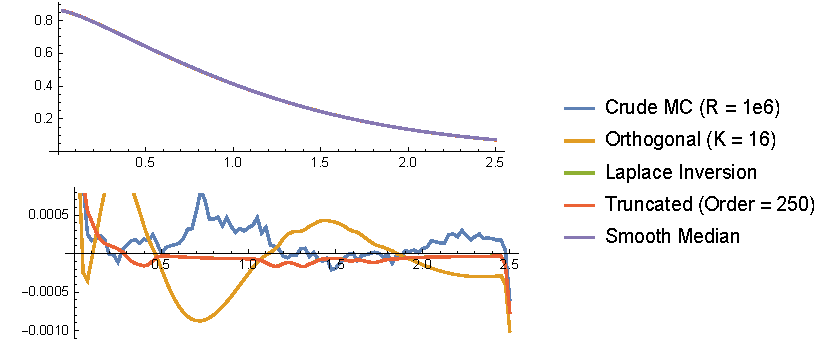
\includegraphics[width=0.95\textwidth]{poisson_gamma_svf.pdf}
\caption{Survival function estimates and approximate absolute error.}
\end{figure}

\begin{figure}[H]
\centering
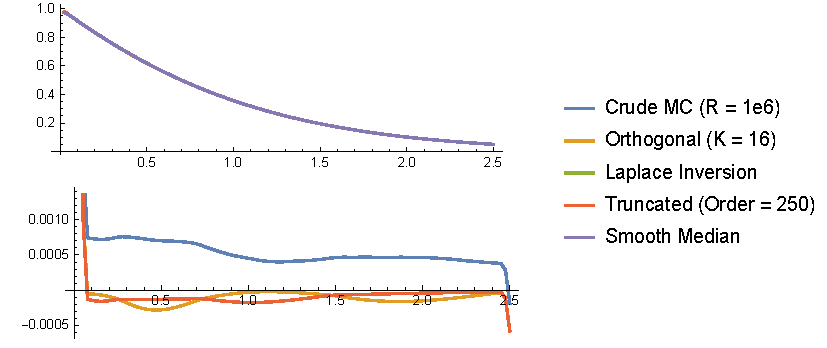
\includegraphics[width=0.95\textwidth]{poisson_gamma_slp.pdf}
\caption{Stop-loss premium estimates and approximate absolute error.}
\end{figure}


\begin{test}
$N\sim\mathsf{Pascal}(\alpha=10,p=1/6)$, and $U\sim\mathsf{Gamma}(r=3/2,m=1/75)$
\end{test}

This test case (up to the scaling constant) has been considered by Jin et al. \cite[Example 3]{JiPrRe16}. In the plots for this test case, the orthogonal estimator, the Laplace inversion estimator, and the truncated estimator all give the same values and hence are hidden underneath the red line for the truncated estimator.

\begin{figure}[H]
\centering
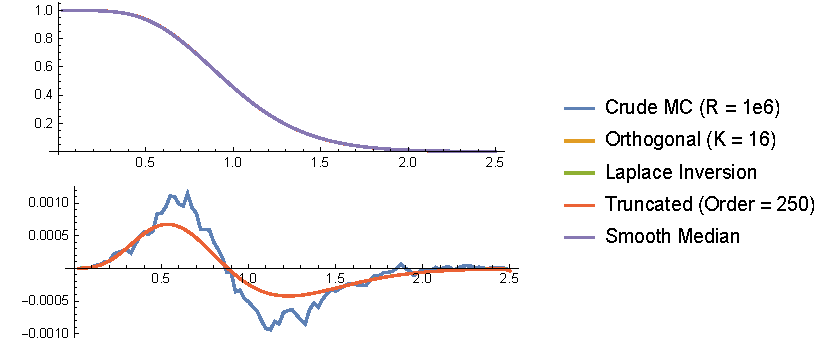
\includegraphics[width=0.95\textwidth]{pascal_gamma_svf.pdf}
\caption{Survival function estimates and approximate absolute error.}
\end{figure}

\begin{figure}[H]
\centering
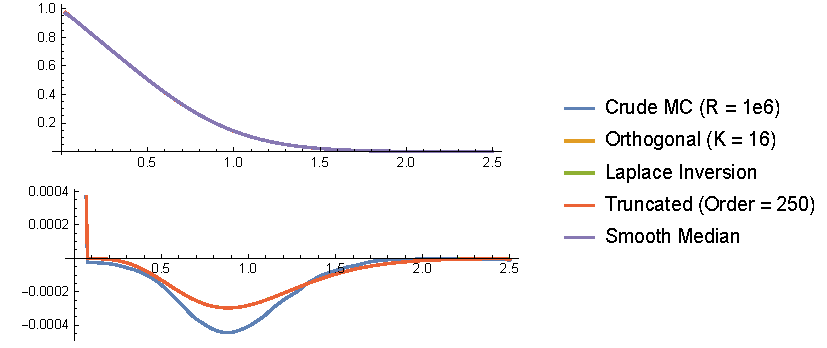
\includegraphics[width=0.95\textwidth]{pascal_gamma_slp.pdf}
\caption{Stop-loss premium estimates and approximate absolute error.}
\end{figure}

\begin{test} $N\sim\mathsf{Poisson}(\lambda=4)$, and $U\sim\mathsf{Pareto}(a=5,b=11,\theta=0)$
\end{test}
The survival function for $U$, given $x \ge \theta=0$, is
\[ \overline{F}_U(x) = \left( 1 + \frac{x-\theta}{a} \right)^{-b} = \left( 1 + \frac{x}{5} \right)^{-11} \,. \]
We note that the Laplace inversion estimator breaks down for small values of $x$ or $a$ in this test case. The specific error given is an ``out of memory'' exception when \textsc{Mathematica} is attempting to do some algebra with extremely large numbers. It is unclear whether a different implementation or selection of parameters would fix this behaviour.

\begin{figure}[H]
\centering
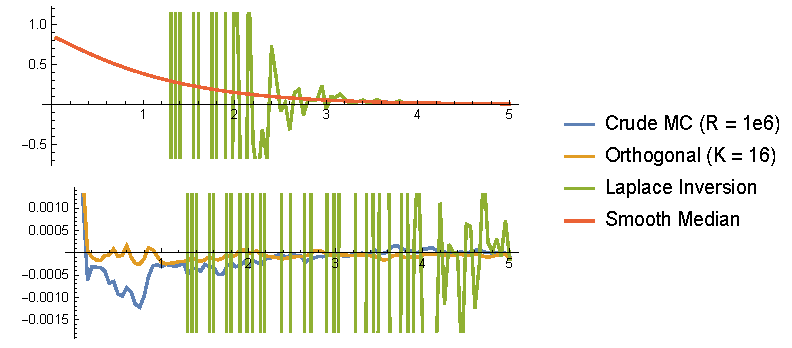
\includegraphics[width=0.95\textwidth]{poisson_pareto_svf.pdf}
\caption{Test 3: Survival function estimates and approximate absolute error.}
\end{figure}

\begin{figure}[H]
\centering
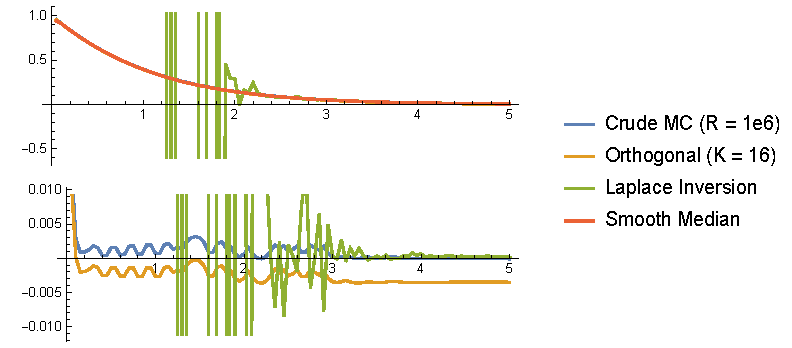
\includegraphics[width=0.95\textwidth]{poisson_pareto_slp.pdf}
\caption{Test 3: Stop-loss premium estimates and approximate absolute error.}
\end{figure}

\begin{test} $N\sim\mathsf{Pascal}(\alpha=2,p=1/4)$, and $U\sim\mathsf{Weibull}(\beta=1/2,\lambda=1/2)$
\end{test}
The survival function for $U$, given $x \ge 0$, is
\[ \overline{F}_U(x) = \exp\left\{ {-} \left(\frac{x}{\lambda} \right)^\beta \right\} = \exp\left\{ {-} \sqrt{2 x}  \right\} \,. \]

\begin{figure}[H]
\centering
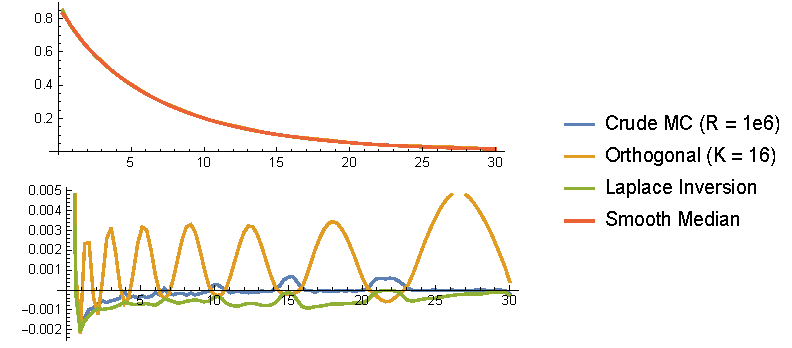
\includegraphics[width=0.95\textwidth]{pascal_weibull_svf.pdf}
\caption{Test 4: Survival function estimates and approximate absolute error.}
\end{figure}

\begin{figure}[H]
\centering
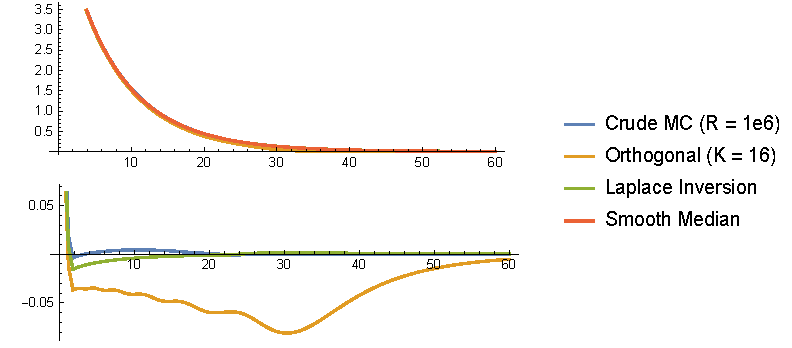
\includegraphics[width=0.95\textwidth]{pascal_weibull_slp.pdf}
\caption{Test 4: Stop-loss premium estimates and approximate absolute error.}
\end{figure}


\subsection{Finite-time ruin probability with no initial reserve} \label{subsec:ApproximationFiniteTimeRuinProbability}

% \begin{test}
% $\lambda=2$, $U\sim\mathsf{Exp}(4)$ and $c=7.2$
% \end{test}


% The finite-time ruin probability is known under a closed form, the expression is given in Albrecher and Asmussen \cite[Chapter 5, Proposition 1.3]{AsAl10}.
In this paper we have used common random numbers for all crude Monte Carlo estimators to smooth their estimates. However in the case of ruin probabilities, the distribution from which we are simulating $\mathrm{Poisson}(\lambda t)$ is changing for each point, so the technique cannot be applied in the traditional way. Thus the crude Monte Carlo estimates in following plots are not as smooth as above. 

\begin{test}
$\lambda=4$ and $U\sim\mathsf{Gamma}(r=2,m=2)$ and $c=1$
\end{test}


\begin{figure}[H]
\centering
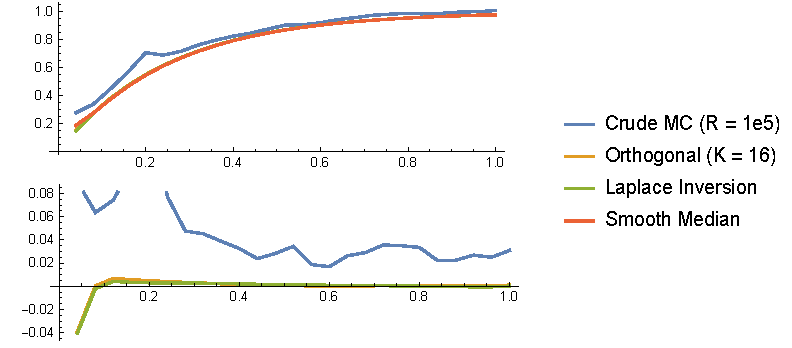
\includegraphics[width=0.95\textwidth]{poisson_exponential_ruin.pdf}
\caption{Test 5: Ruin probability $\psi(0, t)$ estimates and approximate absolute error.}
\end{figure}


% \begin{test}
% $\lambda=1$, $U\sim\mathsf{GPareto}(5,3,1)$, $c=1$

% \end{test}


\begin{test} $\lambda=2$ and $U\sim\mathsf{Pareto}(a=5,b=11,\theta=0)$ and $c=1$
\end{test}

See the discussion of Test 3 for a description of the Laplace inversion estimator's poor behaviour when Pareto variables are involved. 

\begin{figure}[H]
\centering
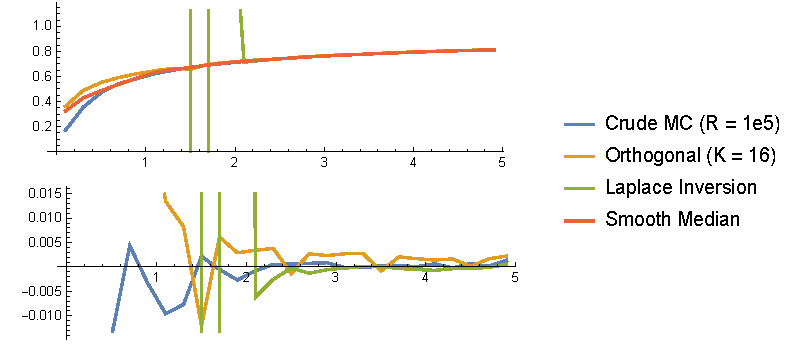
\includegraphics[width=0.95\textwidth]{poisson_pareto_ruin.pdf}
\caption{Test 6: Ruin probability $\psi(0, t)$ estimates and approximate absolute error.}
\end{figure}
\subsection{Concluding remarks}
The orthogonal polynomial method has performed well across all the test cases studied. The accuracy is acceptable even with a rather small order of truncation $K=16$. It produces an approximation having an analytical expression, which is desirable, and in a timely manner. The precision may be improved by adding more terms in the expansions. The main drawback is probably the need for a parametrization tailored to the case studied.\\

The Laplace transform inversion method yields outstanding result in terms of accuracy. It failed to provide a stable approximation for Pareto distributed claim sizes. The parametrization is automatic and seems to fit the different case studied (except the Pareto one).\\

Both of the methods are easy to implement and beat a simple truncation or a crude Monte-Carlo approach, which is the main conclusion of our work.
% \section*{Acknowledgments}  
% Pierre-Olivier Goffard was partially funded by a Center of Actuarial Excellence educational grant given to the University of California, Santa Barbara, by the Society of Actuaries. Patrick J.\ Laub was supported by an Australian Government Research Training Program Scholarship and an Australian Research Council Centre of Excellence for Mathematical \& Statistical Frontiers Scholarship.
%Hereafter a list of examples of combinations of $N$ and $U$ treated in the literature
%\begin{itemize}
%\item In Mnatsakanov and Sarkisian \cite{MnSa13}
%\begin{itemize}
%\item $N\sim\text{Pois}(\lambda)$, $\lambda=2,3$ and $U\sim\mathsf{Exp}(5)$ (parametrized by the mean)
%\[
%\LTsub{S_N}(s) = \exp \Big\{ \frac{-10 s}{1+5s} \Big\} \,, \quad
%\LTsub{S_N}(s) = \exp \Big\{ \frac{-15 s}{1+5s} \Big\} \,.
%\]
%\item $N\sim\text{Pois}(\lambda)$, $\lambda=2,3$ and $U\sim\mathsf{Gamma}(2,5)$ (Sum of two exponential parametrized as above)
%\[
%\LTsub{S_N}(s) = \exp \Big\{ -2 + \frac{2}{(1+5s)^2} \Big\} \,, \quad
%\LTsub{S_N}(s) = \exp \Big\{ -3 + \frac{3}{(1+5s)^2} \Big\} \,.
%\]
%\item $N\sim\text{Pois}(\lambda)$, $\lambda=2,3$ and $U\sim\text{Log-Normal}(0,1)$ .
%\end{itemize}
%\item In Gzyl and Tagliani \cite{GzTa12}
%\begin{itemize}
%\item $N\sim\text{Pois}(1)$, and $U\sim\mathsf{Gamma}(2,1)$
%\[
%\LTsub{S_N}(s) = \exp \Big\{ -1 + \frac{1}{(1+s)^2} \Big\} \,.
%\]
%\item An interesting reference is cited in this paper on the recovery of VAR and TVAR, Patrick could you please look it up and tell me if you thimk this is something we can use. It is a paper of Rockafellar and Uryasev \cite{RoUr00}.
%\end{itemize}
%\item In Provost et al. \cite{GzTa12}
%\begin{itemize}
%\item $N\sim\text{Pois}(3)$, and $U\sim\mathsf{Gamma}(3,2)$
%\[
%\LTsub{S_N}(s) = \exp \Big\{ -3 + \frac{3}{(1 + 2s)^3} \Big\} \,.
%\]
%\item $N\sim\text{Pois}(15)$, and $U\sim\text{IG}(3,2)$.
%\[
%\LTsub{S_N}(s) = \exp \Big\{ 15 \Big[ -1 + \e^{-\frac23 (\sqrt{1+9s}-1)} \Big\} \,.
%\]
%Note that the inverse Gaussian distribution has PDF defined as
%\begin{equation*}
%f(x)=\left(\frac{\theta}{2\pi x^{3}}\right)^{1/2}\exp\left(-\frac{\theta(x-\eta)}{2\eta^{2}x}\right),\text{ }x>0,\text{ }\eta,\theta>0.
%\end{equation*}
%\item $N\sim\mathsf{Pascal}(10,5/6)$, and $U\sim\mathsf{Gamma}(3,2)$, Note that the Pascal distribution $\mathsf{Pascal}(\alpha, p)$ has PMF
%\begin{equation}
%p_N(n)=\binom{\alpha+n-1}{n}(1-p)^{\alpha}p^{n},\text{ }n\geq0\text{ and }0<p<1, \alpha \in \mathbb{N}^{\ast}.
%\end{equation}
%\item $N\sim\mathsf{Pascal}(10,5/6)$, and $U\sim\text{IG}(3,2)$
%\item $N\sim\mathsf{Pascal}(10,5/6)$, and $U\sim\text{Pareto}(3,2)$. Note that the Pareto distribution $\text{Pareto}(\gamma,\delta)$ has PDF
%\begin{equation}
%f(x)=\frac{\gamma \delta^{\gamma}}{(x+\delta)^{\gamma+1}},\text{ }x>0\text{, and }\eta,\delta>0
%\end{equation}
%\end{itemize}
%\item In Dufresne et al. \cite{DuGaMo09},
%\begin{itemize}
%\item $N\sim\text{Pois}(\lambda)$, $\lambda=1,2,3$ and $U\sim\text{GPareto(a,3,1)}$, where $a=4,5,7,10$. Note that the generalized Pareto distribution $GPareto(a,b,\theta)$ has PDF
%\begin{equation}
%f(x)=\frac{1}{B(a,b)}\frac{\theta^{a}x^{b-1}}{(\theta+x)^{a+b}},\text{ }x>0\text{, and }a,b,\theta>0.
%\end{equation}
%\end{itemize}
%\end{itemize}

% \bibliography{TotalClaimAmountApproximationBib}
% \bibliographystyle{plain}
%\appendix
%% \input{Appendix}
%
%\section{Pascal-Exponential sums}
%
%The following lemma, adapted from \cite{PaWi81}, shows a useful correspondence between the Pascal and binomial distributions when used in compound sums with the exponential distribution.
%
%\begin{lemma} \label{lemma:BinomialPascalEquivalence}
%Consider the random sums $X = \sum_{i=1}^{N_1} U_i$ and $Y = \sum_{i=1}^{N_2} V_i$, where
%\[
%N_1 \sim \mathsf{Pascal}(\alpha,p) \,, \quad  U_i \iidDist \mathsf{Exp}(\lambda) \,, \quad  N_2 \sim \mathsf{Binomial}(\alpha,q)  \,, \quad V_i \iidDist \mathsf{Exp}(p \lambda) \,,
%\]
%where $p \in (0,1)$, $\alpha \in \Npos$, $p + q = 1$, and where $\lambda > 0$ is a rate parameter.
%Then we have $X \eqdistr Y$.
%\end{lemma}
%\begin{proof}
%Both $X$ and $Y$ have the same Laplace transform, so $X \eqdistr Y$.
%% The relevant generating functions are
%% $\PGF_{N_1}(t) = \left( \frac{p}{1-qz} \right)^\alpha$ and $\PGF_{N_2}(t) = (p+qz)^\alpha$,
%% and the Laplace transforms of the summands are $\LTsub{U}(t)=\frac{\lambda}{\lambda + t}$ and $\LTsub{V}(t)=\frac{p \lambda}{p\lambda + t}$.
%% So
%% \[
%% \LTsub{X}(t) = \PGF_{N_1}[\LTsub{U}(t)] = \left( \frac{p}{1-q\frac{\lambda}{\lambda + t}} \right)^\alpha
%% =  \left( \frac{p\lambda + p t}{p \lambda + t} \right)^\alpha\,, \text{ and }
%% \]
%% \[
%% \LTsub{Y}(t) = \PGF_{N_2}[\LTsub{V}(t)] = \left(p+q\frac{p \lambda}{p\lambda + t} \right)^\alpha
%% = \left(\frac{p(p\lambda + t) + q p \lambda}{p\lambda + t} \right)^\alpha
%% = \left(\frac{p\lambda + p t}{p\lambda + t} \right)^\alpha
%% \]
%% which implies equality in distribution.
%\end{proof}
%
%% This lemma allows us to reduce infinite summations to finite sums in some cases, like in the following:
%
%\begin{corollary} \label{Coro:PascalExponentialStopLoss}
%Consider the compound sum $S_N = \sum_{i=1}^N U_i$ where $N \sim \mathsf{Pascal}(\alpha,p)$ and the $U_i \iidDist\mathsf{Exp}(\lambda)$.
%Then the \svf of $S_N$ is given by
%\begin{align*}
%\overline{F}_{S_N}(x) &= \sum_{i=1}^\alpha \binom{\alpha}{i} p^i q^{\alpha-i} \e^{-p \lambda x} \sum_{j=0}^{i-1} \frac{(p \lambda x)^j}{j!}
%= \sum_{i=1}^\alpha \binom{\alpha}{i} p^i q^{\alpha-i} \, \Gamma_u(i, p\lambda, x)
%\end{align*}
%and its slp is given by
%\begin{equation}\label{eq:StopLossCompoundNegBinExp}
%\E\left[\left(S_N-a\right)_{+}\right] = \sum_{i=1}^\alpha \binom{\alpha}{i} p^i q^{\alpha-i} \left[ \frac{i}{p \lambda} \Gamma_u\big(i+1, a p \lambda, (a p \lambda)^2 \big) - a \Gamma_u(i, \frac{1}{p \lambda} , a) \right]
%\end{equation}
%\end{corollary}
%\begin{proof}
%By Lemma~\ref{lemma:BinomialPascalEquivalence} we treat $S_N$ as if defined for $N \sim \mathsf{Binomial}(\alpha,q)$ and with $U_i \iidDist \mathsf{Exp}(p \lambda)$.
%The result follows by noting $S_n = U_1 + \dots + U_n \sim \mathsf{Erlang}(n, p \lambda) = \mathsf{Gamma}(n, \frac{1}{p \lambda})$.
%% As $S_n = U_1 + \dots + U_n \sim \mathsf{Erlang}(n, p \lambda) = \mathsf{Gamma}(n, \frac{1}{p \lambda})$ with
%% \[ f_{S_n}(x) = \e^{-p \lambda x} \frac{(p \lambda)^n x^{n-1}}{(n-1)!} = \gamma(n, \frac{1}{p \lambda} , x) \quad\text{and} \quad \overline{F}_{S_n}(x) = \e^{-p \lambda x} \sum_{i=0}^{n-1} \frac{(p \lambda x)^i}{i!} = \Gamma_u(n, \frac{1}{p \lambda} , x) \]
%% and
%% \[ \E[ (S_n - a)_+ ] = \int_a^\infty x f_{S_n}(x) \dd x - a \overline{F}_{S_n}(a)
%% = \frac{n}{p \lambda} \Gamma_u\big(n+1, a p \lambda, (a p \lambda)^2 \big) - a \Gamma_u(n, \frac{1}{p \lambda} , a) \,. \]
%%  % \frac{\gamma(1+n, a p \lambda) - a p \lambda \gamma(n, a p \lambda)}{p \lambda \Gamma(n)} \]
%% Using the law of total expectation we have $f_{S_N}^+(x) = \sum_{i=1}^\alpha \binom{\alpha}{i} q^i p^{\alpha-i} \gamma(i, \frac{1}{p\lambda}, x)$.
%% Selecting $r=1$, $m=1/(p\lambda)$ and $p_i = \binom{\alpha}{i+1} (1-p)^{i+1} p^{\alpha-i-1}$ yields
%% \[ f_{S_N}^+(x) = \sum_{i=0}^{\alpha-1} p_i \gamma(r + i, m, x) \,, \quad \overline{F}_{S_N}(x) = \sum_{i=0}^{\alpha-1} p_i \Gamma_u(r + i, m, x)  \,, \]
%% \[ \E[ (S_N-a)_+] = \sum_{i=0}^{\alpha-1} p_i \Big[ i m \Gamma_u\Big(i+1, \frac{a}{m}, \frac{a^2}{m^2} \Big) - a \Gamma_u(i, m, a) \Big] \,. \]
%\end{proof}
%
%One conclusion of Corollary~\ref{Coro:PascalExponentialStopLoss} is that the exact solution coincides with our approximation with the correct choice of $r$ and $m$ (and with $K \ge \alpha - 1$). Which other choices of $r$, $m$ satisfy the integrability conditions? We can see that
%\[ f_{S_N}^+ = \begin{cases}
%	\Oh( \e^{-\frac{x}{\delta}}) & \text{ as } x \to \infty \text{ for } \delta > (1/p\lambda) \\
%	\Oh( x^\beta ) & \text{ as } x \to 0^+ \text{ for } \beta \le 0
%	\end{cases} \,.
%\]
%so need $m > \delta/2 > 1/(2p\lambda)$, and
%$r \in (0, 2)$.











%!TEX root = ../main.tex
% \chapter{Two numerical methods to evaluate stop-loss premiums}

% \section{Introduction}\label{sec:Introduction}

% Consider the random variable (\rv)
% \begin{equation}\label{eq:AggregatedClaimAmountsRV}
% S_N=\sum_{k=1}^{N}U_{k},
% \end{equation}
% where $N$ is a counting \rv and $\{U_{k}\}_{k\in\N}$ is a sequence of \rvs which are independent and identically distributed (\iid), non-negative, and independent of $N$.
% We denote the probability density function (\pdf) of $S_N$ as $f_{S_N}$, and its survival function (\svf) as
% \begin{equation}\label{eq:DefinitionSurvivalFunction}
% \overline{F}_{S_N}(x)= \P(S_N>x),\quad \text{ for } x\geq0.
% \end{equation}
% This paper concerns approximations of $f_{S_N}$ and $\overline{F}_{S_N}$, though we begin with a discussion of how $S_N$ is used in actuarial science.

% Frequently $S_N$ models the aggregated losses of a non-life insurance portfolio over a given period of time---here $N$ represents the number of claims and $U_k$ the claim sizes---yet other applications also exist. Actuaries and risk managers typically want to quantify the risk of large losses by a single comprehensible number, a risk measure.

% One popular risk measure is the Value-at-Risk (VaR). In actuarial contexts, the VaR at level $\alpha \in (0,1)$ is defined such that the probability of (aggregated) losses exceeding the level VaR is at most $1-\alpha$. We denote this $\alpha$-quantile as
% \begin{equation}
% \text{VaR}_{S_N}(\alpha)=\inf\{x\geq0, F_{S_N}(x)\geq \alpha\}.
% \end{equation}
% Following the European recommendation of the Solvency II directive, the standard value for $\alpha$ is $0.995$, see \cite{EIOPA}. It is used by risk managers in banks, insurance companies, and other financial institutions to allocate risk reserves and to determine solvency margins. Also, we have stop-loss premiums which are risk measures that are commonly used in reinsurance agreements.

% A reinsurance agreement is a common risk management contract between insurance companies, one called the ``cedant'' and the other the ``reinsurer''. Its aim is to keep the cedant's long-term earnings stable by protecting the cedant against large losses. The reinsurer absorbs part of the cedant's loss, say $f(S_N)$ where $0\leq f(S_N)\leq S_N$, leaving the cedant with $I_{f}(S_N)=S_N-f(S_N)$. In return, the cedant pays a premium linked to
% \begin{equation}\label{eq:DefinitionReinsurancePremium}
% \Pi=\E[f(S_N)],
% \end{equation}
% under the expected value premium principle.


% In practice, there are a variety of reinsurance designs from which an insurer can choose. We focus in this work on the stop-loss reinsurance treaty associated to the following ceded loss function
% \begin{equation}\label{eq:StopLossCededFunction}
% f(S_N)=(S_N-a)_{+},\text{ }a\geq0,
% \end{equation}
% where $a$ is referred to as the retention level or priority. The ratemaking of the stop-loss reinsurance policy requires the evaluation of
% \begin{equation}\label{eq:DefUsualStopLossPremium}
% \Pi_{a}(S_N)=\E\left[(S_N-a)_{+}\right],
% \end{equation}
% also known as the usual stop loss premium.

% One variation is the limited stop-loss function,
% \begin{equation}\label{eq:LimitedStopLossCededFunction}
% f(S_N)=\min[(S_N-a)_{+},b],\text{ }a\geq0,
% \end{equation}
% where $b$ is called the limit. The limited stop-loss function \eqref{eq:LimitedStopLossCededFunction} is very appealing in practice because it prevents the cedant from over-estimating their losses and therefore over-charging the reinsurer.
% We also have the change-loss function defined as
% \begin{equation}\label{eq:ChangeLossCededFunction}
% f(S_N)=b(S_N-a)_{+},\text{ }0\leq c\leq1,
% \end{equation}
% which is in between stop-loss and quota-share reinsurance. Note that the ratemaking in each case requires the expectation in \eqref{eq:DefUsualStopLossPremium}.


% From a practical point of view, a reinsurance treaty over the whole portfolio is less expensive to handle than one which involves claim-by-claim management. It also grants protection in the event of an unusual number of claims, triggered for instance by a natural disaster. From a theoretical point of view, it is well known that the stop-loss ceded function allows one to minimize the variance of the retained loss for a given premium level, see for instance the monograph of Denuit et al. \cite{DeDhGoKa06}. Recently, it has been shown that stop-loss reinsurance is also optimal when trying to minimize the VaR and the expected shortfall of the retained loss, see the works of Cai et al. \cite{CaTaWeZh08}, Cheung \cite{Ch10}, and Chi and Tan \cite{ChTa11}. Note that some other ceded loss functions appear in their work, there are however very close to the stop-loss one.

% Unfortunately, one is seriously constrained when calculating these quantities analytically, as there are only a few cases where either the \pdf or the \svf is available in a simple tractable form. To estimate the VaR or stop-loss premium we must find fast and accurate approximations for these functions.

% We discuss the use of an approximation of the \pdf in terms of the gamma density and its orthonormal polynomials. This method has been studied in the recent works of Goffard et al. \cite{GoLoPo15} and Jin et al. \cite{JiPrRe16}. We emphasize here the computational aspect of this numerical method and detail some practical improvements. An exponential change of measure can be used to recover the \pdf of $S_N$ when the claim sizes are governed by a heavy-tailed distribution. This refinement has been successfully applied in the work of Asmussen et al. \cite{AsGoLa16} to recover the density of the sum of lognormally distributed random variables.

% This method is compared to a numerical inversion of the Laplace transform which is known to be efficient to recover the survival function of a compound distribution. The critical step in Laplace inversion is to select which numerical integration technique to apply. We implement a method inspired from the work of Abate and Whitt \cite{Abate1992}, very close to what is proposed in Rolski et al. \cite[Chapter 5, Section 5]{RoScScTe08}. An approximation of the stop-loss premium is then proposed relying on the connection with the survival function of the equilibrium distribution of $S_N$. Note that Dufresne et al. \cite{DuGaMo09} successfully applied a Laplace inversion based technique to the evaluation of stop-loss premium.

% To close, we want to emphasize the fact that the numerical methods apply also in a risk theory framework. The infinite-time ruin probability in the compound Poisson ruin model is equal to the survival function of a compound geometric distribution. The polynomial approximation and the Laplace inversion methods have been employed, and compared to solve this particular problem in the work of Goffard et al. \cite{GoLoPo16}. We add a more original application by noting that the finite-time non-ruin probability with no initial reserves, again under the classical risk model assumptions, may be rewritten as the stop-loss premium associated to a compound Poisson distribution where the priority is expressed in terms of the premium rate and the time horizon.

% The rest of the paper is organized as follows. Section \ref{sec:Preliminaries} introduces compound distributions, and details their role in risk theory. Section \ref{sec:PolynomialApproximation} presents the approximation method based on orthogonal polynomials. Section \ref{sec:NumericalInversionLaplaceTransform} presents the approximation through the numerical inversion of the Laplace transform. Section \ref{sec:NumericalIllustrations} is devoted to numerical illustrations where the performances of the two methods are compared.
%  \section{Compound distributions and risk theory}\label{sec:Preliminaries}

% \framebox{(pjl) Put something here}

% \subsection{Laplace transforms} \label{sec:LaplaceProperties}

% \begin{definition} \label{def:TransformDefs} For a function $f : \R_+ \to \R_+$, we define
% \[
% 	\LT{f}(t) \defeq \int_{0}^{\infty} \e^{-t x} f(x) \dd x\,, \quad \text{for } t \in \C \text{ with } \Re(t) \ge 0 \,, \\
% \]
% to be the corresponding \emph{Laplace transform}.
% For a positive random variable $X$ with \pdf $f_X$, we write $\LTsub{X}(t) \defeq \LT{f_X}(t) = \E\,\e^{-tX}$. \hfill $\diamond$
% \end{definition}

% We have the result that for $t>0$
% \[ \LT{ F_X }(t) = \frac{\LT{f_X}(t)}{t} = \frac{\LTsub{X}(t)}{t} \,, \text{ and } \]
% \[ \LT{ \overline{F}_X }(t) = \frac1t - \LT{F_X(x) }(t) = \frac{1 - \LTsub{X}(t)}{t}  \,. \]
% If we need to consider the defective pdf $f_X^+$, its Laplace transform is related via
% \[ \LTsub{X}(t) = \LT{f_X}(t) = \LT{f_X^+}(t) + \P(X=0) 
% \quad \text{and} \quad
% \LT{F_X^+}(t) = \frac{\LT{f_X^+}(t)}{t}  \,. \]


% \subsection{Compound distribution}
% Let $S_N=\sum_{k=1}^{N}U_k$ be the aggregated claim amounts associated to a non-life insurance portfolio over a fixed time period. The number of claims, also called the claim frequency, is modeled by a counting random variable $N$ having a probability mass function $f_N$. The claim sizes form a sequence $\{U_k\}_{k\in \N}$ of \iid non-negative random variables with common \pdf $f_{U}$. We further assume that the claim sizes are independent from the claim frequency, so the random variable $S_N$ follows the compound distribution $(f_N,f_U)$.

% As $S_N=0$ whenever $N=0$ (assuming this occurs with positive probability), the distribution of $S_N$ is the sum of a singular part (the probability mass $\P(S_N=0)=f_N(0)>0$) and a continuous part (describing $S_N \mid N>0$) with a defective \pdf $f_{S_N}^+$ and \cdf $F_{S_N}^+$. From the law of total probability, we have
% \begin{equation}\label{eq:DefectivePDFCompoundDistribution}
% f_{S_N}^+(x)=\sum_{n=1}^{\infty}f_N(n)f_{U}^{\ast n}(x),~x\geq0.
% \end{equation}

% This density is intractable because of the infinite series. Furthermore, the summands are defined by repeated convolution of $f_{U}$ with itself which is not always straightforward to evaluate. Apart from Panjer's algorithm, the method presented in this work relies on the knowledge of the Laplace transform of $S_N$, which simply involves the Laplace transform of $U$ and the probability generating function of $N$.

% The simple expression of the Laplace transform has made possible the use of numerical methods involving the moments or transform inversion to recover the distribution of $S_N$. The historical competitor of Panjer's algorithm is a Fast Fourier Transform (\fft) algorithm based on the inversion of the discrete Fourier transform. The two methods are compared in the work of Embrechts and Frei \cite{EmFr09}. The polynomial method involves the standard integer moment sequence for $S_N$, in contrast to more exotic types of moments used by some recent methods. Gzyl and Tagliani \cite{GzTa12} uses the fractional moments within a max-entropic based method, while Mnatsakanov and Sarkisian \cite{MnSa13} performs an inversion of the scaled Laplace transform via the exponential moments. In addition to proposing an approximation for the survival function of $S_N$, we provide an efficient way to compute the usual stop-loss premium
% \begin{equation}\label{eq:UsualStopLossPremium}
% \Pi_a(S_N)=\E\left[(S_N-a)_{+}\right],
% \end{equation}
% to allow application to reinsurance.
% \subsection{Risk theory}
% In the classical risk model, the financial reserves of a non-life insurance company are modeled by the risk reserve process $\{R(t),t\geq0\}$, defined as
% \begin{equation}\label{eq:RiskReserveProcess}
% R(t)=u+ct-\sum_{k=1}^{N(t)}U_k.
% \end{equation}
% The insurance company holds an initial capital of amounts $R(0)=u\geq0$, and collects premiums at a constant rate of $c\geq0$ per unit of time. The number of claims up to time $t\geq0$ is governed by a homogeneous Poisson process $\{N(t),t\geq0\}$ with intensity $\lambda$. The claim sizes are \iid non-negative random variables independent from $N(t)$.

% One of the goals of risk theory to evaluate an insurer's ruin probability, that is, the probability that the financial reserves eventually fall below $0$. Of interest are both the finite-time ruin probability $\psi(u,T)$ and the infinite-time ruin probability, also called the \emph{probability of ultimate ruin}, $\psi(u)$, which are defined as
% \begin{equation}\label{eq:FiniteTimeRuinProbability}
% \psi(u,T)=\P\Big( \inf_{0 \le t \le T} R(t) \leq 0 \Big),
% \end{equation}
% and
% \begin{equation}\label{eq:InfiniteTimeRuinProbability}
% \psi(u)=\P\Big( \inf_{t \geq 0}\,R(t) \leq 0 \Big).
% \end{equation}
% These probabilities are often reformulated (for mathematical convenience) in terms of the associated claims surplus process $\{S(t),t\geq0\}$,
% \begin{equation} \label{eq:ClaimsSurplusProcess}
% S(t) = \sum_{k=1}^{N(t)} U_k - ct,\text{ }t\geq0,
% \end{equation}
% specifically,
% \begin{equation}
% \psi(u,T)=\P\Big( \sup_{0 \le t \le T} S(t) \geq u \Big) \quad \text{and} \quad
% \psi(u)=\P\Big( \sup_{t \geq 0}\,S(t) \geq u \Big).
% \end{equation}

% For a general background on risk theory and the evaluation of ruin probabilities, we refer the reader to the monograph of Asmussen and Albrecher \cite{AsAl10}.

% The first connection between compound distributions and ruin probabilities is the following.
% If the net benefit condition is satisfied, \ie if the premium rate exceeds the average cost of aggregated claims per unit of time, then the infinite-time ruin probability is given by the survival function of a geometric compound distribution. More precisely,
% \begin{equation}\label{eq:PollaczeckKhinchineFormula}
% \psi(u) = \P\left(S_N \defeq \sum_{k=1}^{N}V_{k}>u\right)
% = (1 - \rho) \sum_{n=1}^\infty \rho^n \overline{F}_V^{\ast n}(u),
% \end{equation}
% with $N \sim \mathsf{Geom}_0(\rho)$, $\rho = \lambda\E(U)/c$, and with \iid $V_{k}$ with \pdf $f_{V}(x)= \overline{F}_U(x) / \E(U)$. This result is known as the Pollaczeck--Khinchine formula, see for instance Asmussen and Albrecher \cite[Chapter IV, (2.2)]{AsAl10}. Thus it is possible to evaluate the infinite-time ruin probability via Panjer's algorithm. If we are able to determine the Laplace transform of $V$ then we can also apply the polynomial method of Goffard et al. \cite{GoLoPo15}, the fractional moment based method of Gzyl et al. \cite{GzNITa13}, and the exponential moments based method of Mnatsakanov et al. \cite{MnSaHa15}.

% The second connection links the finite-time ruin probability with no initial reserves to the stop-loss premium associated with a compound distribution. 
% For now, consider $N(t) \sim \mathsf{Poisson}(\lambda t)$ (\ie the claims arrive as a homogeneous Poisson process), and so Cram\'{e}r's formula (given for $c=1$ in \cite[Chapter V Theorem 2.1]{AsAl10}, and for $c>0$ in \cite[Theorem 2]{michna2010ruin}) tells us that
% \begin{align} \label{CramersFormula}
% \psi(0, T)
% &= 1 - \frac{1}{cT} \int_0^{cT} \P \Big( \sum_{i=1}^{N(T)} U_i \le x \Big) \dd x \,.
% \end{align}
% Writing $S_{N_T} = \sum_{i=1}^{N(T)} U_i$ we can see that \eqref{CramersFormula} says that $\psi(0,T) = \E [ \min\{S_{N_T}, cT \} ]/cT$ and hence
% \begin{align} \label{eq:ConnectionFiniteTimeRuinProbabilityStopLossPremium}
% \psi(0, T)
% &= (cT)^{-1} \Big[  \E[N_T] \, \E[U_1] - \Pi_{cT}(S_{N_T}) \Big] \,.
% \end{align}
% Lef\`evre and Picard \cite[Corollary 4.3]{LePi11} show that equations \eqref{CramersFormula} and \eqref{eq:ConnectionFiniteTimeRuinProbabilityStopLossPremium} hold for more general cases. In particular, the result holds when the claim arrival process forms a \emph{homogeneous point processes} (\cf Definition~\ref{def:HomogeneousPointProcess}) and even when the claim sizes are interdependent. This allows us to use \eqref{eq:ConnectionFiniteTimeRuinProbabilityStopLossPremium} in cases then $N(T)$ has any non-negative discrete distribution.

% \begin{definition} \label{def:HomogeneousPointProcess}
% A point process on $[0, T]$ is a \emph{homogeneous point process} \cite{de1999inequality,LePi11} if for all $n > 0$ we have
% \[ (N(s) \mid N(t) = n) \sim \mathsf{Binomial}\big(n, \frac{s}{t} \big) \,. \]
% This generalises the standard Poisson process by allowing the distribution of $N(T)$ to be arbitrary.
% Theorem~A2 of \cite{de1999inequality} shows that any homogeneous point process on $[0,\infty)$ is a mixed Poisson process.
% \end{definition} \section{Orthogonal polynomial approximations}\label{sec:PolynomialApproximation}

% \subsection{Approximating general density functions} \label{ssec:PolynomialApproxIntro}
% Let $X$ be an arbitrary random variable with \pdf\footnote{This section is written from the perspective of approximating a \pdf, however the main results also hold if applied to a defective density.} $f_X$ with respect to some measure $\lambda$ (typically Lebesgue measure on an interval or counting measure on a subset of $\Z$). We assume that the density is unknown and we propose an approximation of the form
% \begin{equation}\label{eq:PolynomialApproximation}
% \widehat{f}_{X}(x)=\sum_{k=0}^{K}q_{k}Q_{k}(x)f_{\nu}(x).
% \end{equation}
% where $f_{\nu}$ is the reference or basis density, associated to a probability measure $\nu$ absolutely continuous with respect $\lambda$. The sequence $\{Q_{k},k \geq 0\}$ is made of polynomials, orthonormal with respect to $\nu$ in the sense that
% \begin{equation}\label{eq:OrthonormalProperty}
% \left<Q_{k},Q_{l}\right>_\nu =\int Q_{k}(x)Q_{l}(x)\dd\nu(x)= \delta_{k,l},\text{ }k,l\in\N.
% \end{equation}
% This sequence is generated by the Gram--Schmidt orthogonalization procedure 
% which is only possible if $\nu$ admits moments of all orders. If additionally there exists $s>0$ such that
% \begin{equation}
% \int \e^{sx}\dd\nu(x)<\infty\nonumber
% \end{equation}
% then the sequence of polynomials $\{Q_{k},k \geq 0\}$ forms an orthonormal basis of $\Lp^2(\nu)$ which is the space of all square integrable functions with respect to $\nu$, see the monograph by Nagy \cite[Chapter 7]{Na65}. Therefore, if $f_{X}/f_{\nu}\in \Lp^2(\nu)$ then the polynomial representation of the density of $X$ with respect to $\nu$ follows from orthogonal projection, namely we have
% \begin{equation}\label{eq:PolynomialRepresentationTheory}
% f_{X}(x)/f_{\nu}(x)=\sum_{k=0}^{\infty}\left<f_{X}/f_{\nu} , Q_{k}\right>_\nu Q_{k}(x).
% \end{equation}
% We label the coefficients of the expansion as $\{q_{k},k \geq 0\}$, noting that
% \begin{equation}
% q_k\defeq \left<f_{X}/f_{\nu} , Q_{k}\right>_\nu =\int Q_{k}(x)f_{X}(x)\frac{\dd \nu(x)}{f_\nu(x)} =\E\left[Q_{k}(X)\right], \text{ }k\in \N,\nonumber
% \end{equation}
% and thus we can rearrange \eqref{eq:PolynomialRepresentationTheory} to be
% \begin{equation}\label{eq:PolynomialRepresentation}
% f_{X}(x)=\sum_{k=0}^{\infty} q_k Q_{k}(x) f_{\nu}(x).
% \end{equation}
% The approximation \eqref{eq:PolynomialApproximation} follows by simply truncating the series to $K+1$ terms.

% The Parseval relationship, $\sum_{k=1}^{\infty}q_{k}^{2}=||f_{X}/f_{\nu}||_\nu^{2}$, ensures that the sequence $\{q_{k},k \geq 0\}$ tends toward $0$ as $k$ tends to infinity. The accuracy of the approximation \eqref{eq:PolynomialApproximation}, for a given order of truncation $K$, depends on how swiftly these coefficients decay. The $\Lp^2$ loss associated with the approximation of $f_{X}/f_{\nu}$ is $\sum_{k=K+1}^{\infty}q_{k}^{2}$.

% Typical choices of reference distributions are ones that belong to a Natural Exponential Family with Quadratic Variance Function (NEF-QVF) which includes the normal, gamma, hyperbolic, Poisson, binomial, and negative binomial distributions.
% This family of distributions is convenient as the associated orthogonal polynomials are classical, see the characterization by Morris \cite{Mo82}. The polynomials are known explicitly, thus we avoid the time-consuming Gram--Schmidt orthogonalization procedure. Furthermore, it has been shown in a paper by Provost \cite{Pr05} that the recovery of unknown densities from the knowledge of the moments of the distribution naturally leads to approximation in terms of the gamma density and Laguerre polynomials when $X$ admits $\R_{+}$ as support, and in terms of the normal density and Hermite polynomials when $X$ has $\R$ as support.

% \subsection{Approximating densities of positive random variables} \label{ssec:PolynomialApproxPositive}

% To approximate the \pdf for positive $X$, a natural candidate for the reference density is the gamma density. It has been proven to be efficient in practice, see the work of Goffard et al. \cite{GoLoPo15,GoLoPo16}, and Jin et al. \cite{JiPrRe16}. The work of Papush et al. \cite{PaPaPo01} showed that among the gamma, normal and lognormal distribution, the gamma distribution seems to be better suited to model certain aggregate losses. The lognormal distribution is a problematic choice. Even though the orthogonal polynomials are available in a closed form see Asmussen et al. \cite{AsGoLa16}, they do not provide a complete orthogonal system of the $\Lp^2$ space. The case of the inverse Gaussian as basis received a treatment in the work of Nishii \cite{Ni96}, where it is shown that the only way to get a complete system of polynomials is by using the Gram--Schmidt orthogonalization procedure. Differentiating the density (as it is done in the case of NEF-QVF) does not lead to an orthogonal polynomial system, and starting from the Laguerre polynomials leads to a system of orthogonal functions which is not complete. A solution might be to exploit the bi-orthogonality property pointed out in the work of Hassairi and Zarai \cite{HaZa04}. To close this review of reference densities, we mention the work of Nadarajah et al. \cite{NaChJi16} where Weibull and exponentiated exponential distributions are considered as reference density.

% The $\mathsf{Gamma}(r,m)$ distribution, where $r$ is the shape parameter and $m$ is the scale parameter, has a \pdf
% \begin{equation}\label{eq:PDFGamma}
% f_\nu(x)\defeq\gamma(r,m,x)=\frac{x^{r-1}\e^{-\frac{x}{m}}}{\Gamma(r)m^{r}},\text{ }x\in\R^{+},
% \end{equation}
% where $\Gamma(\cdot)$ denotes the gamma function. 
% The associated orthonormal polynomials are given by
% \begin{equation}\label{eq:GeneralizedLaguerrePolynomials}
% Q_{n}(x)
% =(-1)^{n} \binom{n + r - 1}{n}^{-\frac12} L_{n}^{r-1}\big(\frac{x}{m}\big)
% =(-1)^{n} \left( \frac{\Gamma(n+r)}{\Gamma(n+1)\Gamma(r)} \right)^{-\frac12} L_{n}^{r-1}\big(\frac{x}{m}\big),
% \end{equation}
% where $\{L_{n}^{r-1},n\geq0\}$ are the generalized Laguerre polynomials,
% \begin{equation}\label{eq:GeneralizedLaguerrePolynomialsExpression}
% L_{n}^{r-1}(x)
% =\sum_{i=0}^{n} \binom{n + r - 1}{n - i} \frac{(-x)^i}{i!}
% =\sum_{i=0}^{n} \frac{\Gamma(n+r)}{\Gamma(n-i+1)\Gamma(r+i)}\frac{(-x)^i}{i!}, \text{ }n\geq 0,
% \end{equation}
% cf. the classical book by Szeg{\"o} \cite{Sz39}. 

% \begin{Lemma}\label{Lemma:PseudoMixtureOfGammas}
% If $\nu$ is $\mathsf{Gamma}(r,m)$, the polynomial expansion \eqref{eq:PolynomialRepresentation}  may be rewritten as
% \begin{align}\label{eq:PseudoMixtureOfGammas}
% f_{X}(x)&= \sum_{i=0}^{\infty} p_i \gamma(r+i,m,x), 
% \end{align}
% where
% \begin{equation}\label{eq:PiExpression}
% p_i 
% =\sum_{k=i}^\infty q_k \frac{(-1)^{i+k}}{i! \, (k-i)!} \sqrt{\frac{k! \Gamma(k+r)}{\Gamma(r)}}
% \end{equation}

% and the function $\gamma(r,m,x)$ is the \pdf of the $\mathsf{Gamma}(r,m)$ distribution.
% \end{Lemma}
% \begin{proof}
% If we change the sum from iterating over Laguerre polynomials to iterating over monomials we get
% \[
% f_{X}(x)=\sum_{k=0}^{\infty} q_k Q_{k}(x) f_{\nu}(x) = \sum_{i=0}^\infty c_i x^i \gamma(r,m,x) \,
% \]
% where
% \begin{align*}
% c_i
% &= \sum_{k=0}^\infty \text{Coefficient}(x^i, q_k  Q_k(x)) 
% = \frac{(-1)^i}{m^i i!} \sum_{k=i}^\infty q_k (-1)^{k} \binom{k + r - 1}{k}^{-\frac12} \binom{k + r - 1}{k - i} \,.
% \end{align*}
% We also note that
% \[ x^i \gamma(r, m, x) = m^i \frac{\Gamma(r+i)}{\Gamma(r)} \gamma(r+i, m, x) \]
% so
% \[ f_{X}(x) = \sum_{i=0}^\infty c_i m^i \frac{\Gamma(r+i)}{\Gamma(r)} \gamma(r+i, m, x) =  \sum_{i=0}^\infty p_i \gamma(r+i, m, x)  \]
% where we have set $p_i = c_i m^i \Gamma(r+i) / \Gamma(r)$. 
% \end{proof}

% \begin{remark}
% For $r=1$, the formula for $p_i$, \eqref{eq:PiExpression}, simplifies to
% \[ p_i = \sum_{k=i}^\infty q_k (-1)^{i+k} \binom{k}{i} \,. \]
% \end{remark}

% The expression \eqref{eq:PseudoMixtureOfGammas} resembles a mixture of Erlang distributions, which are extensively used for risk modeling purposes, \cf Willmot and Woo \cite{WiWo07}, Lee and Lin \cite{LeLi10}, and Willmot and Lin \cite{WiLi11}. However, the $p_i$'s defined in \eqref{eq:PiExpression} does not form a proper probability mass function as they are not always positive. Hence our approximation cannot be considered as an approximation through an Erlang mixture.  



% \subsection{Approximating densities of positive compound distributions}

% We now focus on variables $S_N$ which are compound distributed. Since these distributions have an atom at 0, we put aside this singularity and focus on the defective \pdf $f_{S_N}^+$.
% The discussion in Subsections \ref{ssec:PolynomialApproxIntro} and \ref{ssec:PolynomialApproxPositive} also apply to defective densities.



% If $f_{S_N}^+/f_{\nu}\in\Lp^2(\nu)$ then we have
% \begin{equation}\label{eq:PseudoErlangMixtureRepresentationDefectivePDF}
% f_{S_N}^+(x)= \sum_{k=0}^\infty q_k Q_k(x) \, \gamma(r, m, x) = \sum_{i=0}^{\infty} p_i \gamma(r+i,m,x),\text{ for }x>0,
% \end{equation}
% where $q_k=\int_{0}^{\infty}Q_{k}(x)f_{S_N}^+(x)\dd x$ and $p_i$ is given by \eqref{eq:PiExpression}.
% Truncating the first summation yields
% \begin{equation}\label{eq:ApproxPolynomialRepresentation}
% f_{S_N}^{+}(x)
% \approx \sum_{k=0}^{K} q_k Q_{k}(x) \, \gamma(r,m,x)
% = \sum_{i=0}^{K} \widehat{p}_i\gamma(r+i,m,x)
% \end{equation}
% where $\widehat{p}_i =\sum_{k=i}^K q_k (-1)^{i+k} / [i! \, (k-i)! ] \sqrt{k! \Gamma(k+r) / \Gamma(r)}$ for $i \le K$.
% A sufficient condition for $f_{S_N}^+/f_{\nu}\in\Lp^2(\nu)$ is
% \begin{equation}\label{eq:IntegrabilityCondition}
% f_{S_N}^+(x)=
% \begin{cases}
% \Oh(\e^{- x/\delta})&\text{ as }x\rightarrow\infty\text{ with }m>\delta/2,\\
% \Oh(x^{\beta})&\text{  as }x\rightarrow0\text{ with } r < 2( \beta + 1).
% \end{cases}
% \end{equation}

% When $S_N$ has a well-defined moment generating function one can typically choose $r$ and $m$ so this integrability condition is satisfied. However this is not true when we consider claim sizes from heavy-tailed distributions, which is a desirable model characteristic. When the integrability condition cannot be satisfied, the work-around is to use the expansion
% \[ \e^{-\theta x} f_{S_N}^{+}(x) 
% = \sum_{k=0}^\infty q_k Q_k(x) f_\nu(x)  \]
% for some $\theta > 0$. Thus, we can use
% \begin{align*}
% f_{S_N}^+(x)
% &= \e^{\theta x} \sum_{k=0}^\infty q_k Q_k(x) f_\nu(x)
% =  \e^{\theta x} \sum_{i=0}^{\infty} p_i \gamma(r+i,m,x)
% \end{align*}
% and since
% \[ \e^{\theta x} \gamma(r+i, m, x) = (1-m \theta)^{-(r+i)} \gamma\big(r+i, \frac{m}{1-m\theta}, x \big)  \]
% we have
% \begin{align}
% f_{S_N}^+(x)
% = \sum_{i=0}^{\infty} p_i (1-m \theta)^{-(r+i)} \gamma\big(r+i, \frac{m}{1-m\theta}, x \big)
% = \sum_{i=0}^{\infty} \widetilde{p}_i \gamma\big(r+i, \widetilde{m}, x \big)
% \end{align}
% where
% \[ \widetilde{p}_i = \frac{ p_i }{(1-m \theta)^{r+i}} 
% \quad\text{and}\quad
% \widetilde{m} = \frac{m}{1-m\theta} \,.
% \]
% Calculating the $q_i$'s and $p_i$'s is a topic we will cover in Section~\ref{ssec:ComputingOrthogonalCoefficients}, but it requires a Laplace transform of $\e^{-\theta x} f_{S_N}^{+}(x)$. This is
% \begin{align*}
% \LT{ \e^{-\theta x} f_{S_N}^{+}(x) }(t)
% = \LT{ f_{S_N}^+(x) }(t+\theta) 
% = \LTsub{ S_N }(t+\theta) - f_N(0)
% \end{align*}

% The method described above is the same (up to some constants) as approximating the exponentially tilted distribution.
% This idea has been used in Asmussen et al. \cite{AsGoLa16}. 
% It is easily seen that taking $1/\theta >  m >1/2\theta$ implies that $(\e^{-\theta x} f_{S_N}^+(x))/f_{\nu}(x)\in\Lp^2(\nu)$.

% \begin{color}{brown}
% We could add here a treatment of the Inverse Gaussian case maybe...
% \end{color}



% The next section shows that our approximation allows a quick evaluations of survival function and stop-loss moments, see Proposition \ref{prop:OrthogonalPolynomialForm}.

% \subsection{Polynomial approximation of the survival function and the stop-loss premium}

% In this section, we exploit Lemma~\ref{Lemma:PseudoMixtureOfGammas} to provide a formula for the different quantities of interest mentioned in the introduction, namely the \cdf, the tail function the usual stop-loss premium and the practical stop-loss premium of $S_N$. The formulas give rise to approximation based on gamma related special functions available as built-in function in computational software such as \texttt{Mathematica}.
% \begin{proposition} \label{prop:OrthogonalPolynomialForm}
% \begin{itemize}
% \item[(i)] The \svf of $S_N$ is given by
% \begin{equation}\label{eq:TailFunctionX}
% \overline{F}_{S_N}(x) = \sum_{i=0}^{\infty}p_i\Gamma_{u}(r+i,m,x) \quad \text{for } x \ge 0 \,.
% \end{equation}
% \item[(ii)] The usual stop-loss premium of priority $a \ge 0$, associated to $S_N$, is given by
% \begin{equation}
% \E\left[\left(S_N-a\right)_{+}\right] = \sum_{i=0}^{\infty}p_i\left[m (r+i) \Gamma_{u}(r+i+1,m,a)-a\Gamma_{u}(r+i,m,a)\right]. \label{eq:UsualStoplossX} 
% \end{equation}
% \end{itemize}
% The function $\Gamma_u(r,m,x)$ corresponds to the \svf of the $\mathsf{Gamma}(r,m)$ distribution.
% \end{proposition}
% \begin{proof}
% The probability measure of $S_N$ admits a singular part and a continuous part. Namely, we have
% \begin{equation*}\label{eq:ProbabilityMeasureX}
% \dd\P_{S_N}(x)=f_{N}(0)\delta_0(x)+f_{S_N}^+(x)\dd\lambda(x),\text{ }x\in\R_{+},
% \end{equation*}
% where $\delta_0$ denotes the Dirac measure at $0$ and $\lambda$ the Lebesgue measure on $\R_{+}$. If $f_{S_N}^+/f_\nu\in \Lp^2(\nu)$ then applying \eqref{eq:PseudoMixtureOfGammas} from Lemma~\ref{Lemma:PseudoMixtureOfGammas} allows to rewrite $f_{S_N}^+$ as
% \begin{equation}\label{eq:PolynomialRepresentationRewrittenProp}
% f_{S_N}^+(x)=\sum_{i=0}^{\infty} p_i \gamma(r+i,m,x).
% \end{equation}
% Integrating the probability measure of $S_N$ on $\left[x,\infty\right)$ yields the formula \eqref{eq:TailFunctionX}.
% Consider the usual stop-loss premium of $S_N$, and note that
% \begin{align}
% \E\left[(S_N-a)_+\right]=&\int_{0}^{\infty}(x-a)_{+}\dd\P_{S_N}\nonumber\\
% =&\int_{a}^{\infty}(x-a)f_{S_N}^+(x)\dd x \nonumber\\
% =&\int_{a}^{\infty}xf_{S_N}^+(x)\dd x-a\overline{F}_{S_N}(a).\label{eq:UsualStopLossXProof1}
% \end{align}
% Then notice that for every $i \in \N$, we have that
% \begin{align}
% \int_{a}^{\infty} x \, \gamma(r+i, m, x)\dd x
% &= \int_{a}^{\infty}x\frac{x^{r+i-1} \e^{-x/m}}{\Gamma(r+i)m^{r+i}}\dd x\nonumber\\
% &= m\frac{\Gamma(r+i+1)}{\Gamma(r+i)}\int_{a}^{\infty}\frac{x^{r+i} \e^{-x/m}}{\Gamma(r+i+1)m^{r+i+1}}\dd x\nonumber\\
% &= m (r+i) \Gamma_{u}(r+i+1,m,a).\label{eq:UsualStopLossXProof2}
% \end{align}
% Therefore substituting \eqref{eq:PolynomialRepresentationRewrittenProp} into \eqref{eq:UsualStopLossXProof1} and simplifying with \eqref{eq:UsualStopLossXProof2} yields \eqref{eq:UsualStoplossX}.
% \end{proof}

% \subsection{Computation of the coefficient of the polynomial expansion} \label{ssec:ComputingOrthogonalCoefficients}


% The inherent challenge of the implementation of the polynomial method remains the evaluation of the coefficients $\{q_k, k\geq0\}$. Recall that
% \begin{equation*}
% q_{k}=\int_{0}^{\infty}Q_k(x)f_{S_N}^+(x)\dd x,\text{ }k\geq0,
% \end{equation*}
% we propose an evaluation based on the Laplace transform $\LT{f_{S_N}^+}$. Define the generating function of the sequence $\{q_k c_k, k\geq0\}$ as $\mathcal{C}(z)=\sum_{k=0}^{\infty}q_{k}c_{k}z^{k}$, where
% \begin{equation}\label{eq:ck}
% c_k= \left(\frac{\Gamma(k+r)}{\Gamma(k+1)\Gamma(r)}\right)^{1/2} \quad \text{ for }k\geq0 \,.
% \end{equation}
% The following result establishes a link between the Laplace transform of $f_{S_N}^+$  and the generating function $\mathcal{C}(z)$.
% \begin{proposition}\label{prop:LaplaceTransformPolynomialRepresentation}
% Assume that $f_{S_N}^+/f_{\nu}\in\Lp^{2}(\nu)$, then we have
% \begin{equation}\label{eq:CoefficientGeneratingFunctionToLaplaceTransforn}
% \mathcal{C}(z)=(1+z)^{-r}\LT{f_{S_N}^+}\Big[\frac{-z}{m(1+z)}\Big].
% \end{equation}
% \end{proposition}
% \begin{proof}
% As $f_{S_N}^+/f_{\nu}\in\Lp^{2}(\nu)$, the polynomial representation of $f_{S_N}^+$ follows from the application of Lemma~\ref{Lemma:PolynomialRepresentation} with
% \begin{equation}\label{eq:prop:PolynomialRepresentationgX}
% f_{S_N}^+(x)=\sum_{k=0}^{\infty}\sum_{i=0}^{k}q_k\tilde{q}_{i,k}(r)\gamma(r+i,m,x).
% \end{equation}
% Taking the Laplace transform in \eqref{eq:prop:PolynomialRepresentationgX} yields
% \begin{align}
% \LT{f_{S_N}^+}(s)
% &= \sum_{k=0}^{\infty}\sum_{i=0}^{k}q_k\tilde{q}_{i,k}(r)\left(\frac{1}{1+sm}\right)^{r+i}\nonumber\\
% &= \left(\frac{1}{1+sm}\right)^{r}\sum_{k=0}^{\infty}q_k \sum_{i=0}^{k} (-1)^{k+i} \left(\frac{\Gamma(k+r)}{\Gamma(k+1)\Gamma(r)}\right)^{1/2} \binom{k}{i} \left(\frac{1}{1+sm}\right)^{i}\nonumber \\
% &= \left(\frac{1}{1+sm}\right)^{r}\sum_{k=0}^{\infty}q_k c_k (-1)^{k} \sum_{i=0}^{k} \binom{k}{i} \left(\frac{-1}{1+sm}\right)^{i} \nonumber\\
% &= \left(\frac{1}{1+sm}\right)^{r}\sum_{k=0}^{\infty}q_k c_k (-1)^{k} \left( \frac{sm}{1+sm}  \right)^{k}\nonumber \\
% &= \left( 1 - \frac{sm}{1+sm}\right)^{r}\mathcal{C}\left(-\frac{sm}{1+sm}\right).\label{eq:LaplaceTransfornToCoefficientGeneratingFunction}
% \end{align}
% Thus \eqref{eq:CoefficientGeneratingFunctionToLaplaceTransforn} follows from letting $z= -sm / (1+sm)$.
% \end{proof}

% The coefficients of the polynomials can be derived after differentiation of the generating function $\mathcal{C}(z)$ as
% \begin{align}\label{eq:PolynomialExpansionCoefficientDerivativeGeneratingFunction}
% q_k&=\frac{1}{c_k}\frac{1}{k!}\frac{\dd^{k}}{\dd z^{k}}\mathcal{C}(z)\Big\rvert_{z=0}  =\frac{1}{c_k} \text{Coefficient}(k, \text{MaclaurinSeries}(\mathcal{C}(z)))
% \end{align}

% \framebox{Below is the version for the $p_i$'s}

% The inherent challenge of the implementation of the polynomial method remains the evaluation of the coefficients $\{p_i, i\geq0\}$. Assuming that $f_{S_N}^+/f_{\nu}\in\Lp^2(\nu)$ then taking the Laplace transform on both side of \eqref{eq:PseudoErlangMixtureRepresentationDefectivePDF} yields
% \begin{eqnarray}
% \LT{f_{S_N}^+}(s)&=&\sum_{i=0}^{\infty} p_i \left(\frac{1}{1+sm}\right)^{r+i}\nonumber\\
% &=&\left(\frac{1}{1+sm}\right)^{r}\mathcal{C}\left(\frac{1}{1+sm}\right),\label{eq:PseudoErlangMixtureLaplaceTransform}
% \end{eqnarray}
% where $\mathcal{C}(z)=\sum_{i=1}^{\infty}p_i z^{i}$ denotes the generating function of the sequence of coefficient $\{p_i\text{ , }i\geq1\}$. Now setting $z=\frac{1}{1+sm}$ allows to express the generating function $\mathcal{C}(z)$ in terms of the Laplace transform of $S_N$ as 
% \begin{equation}\label{eq:GeneratingFunctionPi}
% \mathcal{C}(z)=z^{-r}\LT{f_{S_N}^+}\left(\frac{1-z}{zm}\right).
% \end{equation}
% The coefficients of the polynomials can be derived after differentiation of the generating function $\mathcal{C}(z)$ as
% \begin{align}\label{eq:PolynomialExpansionCoefficientDerivativeGeneratingFunction}
% p_i&=\frac{1}{k!}\frac{\dd^{k}}{\dd z^{k}}\mathcal{C}(z)\Big\rvert_{z=0}  =\text{Coefficient}(k, \text{MaclaurinSeries}(\mathcal{C}(z)))
% \end{align}
% for $i\geq0$. \begin{color}{brown} There I am worried about the singularities at $0$ in the function $\mathcal{C}(z)$, then the derivative might admits singularities as well. I don't understand why we have singularities for the computations of the $p_i$'s while the computation of the $q_k$'s does not seem to cause those problems.
% \end{color}
% \begin{remark}
% The approximation through an Erlang mixture consists in approximating the \pdf of a nonnegative random variable $X$ as 
% \begin{equation}\label{eq:ErlangMixtureRepresentation}
% f_X(x)=\sum_{i=1}^{\infty}p_i\gamma(i,m,x),\text{ for }x\geq0.
% \end{equation}
% The function $\mathcal{C}(z)$ becomes then the probability generating function (\pgf) of a counting random variable $N$, where $p_i=\mathbb{P}(N=i),\text{ for }i\geq1$.
% \end{remark}
% A good choice of the parameters $m$ amd $r$ of the baseline density may help enhancing the convergence of our approximation by making the shrinkage of the expansion coefficient faster. The next example is designed to shed light on the link between our polynomial expansion and an Erlang mixture.

% \begin{example}\label{ex:RecoveryExponentialRV}
% Suppose that we are interested in approximating the \pdf of an exponential random variable $\text{Exp}(\beta)$. The generating function of the coefficients is then 
% \begin{equation}\label{eq:GeneratingFunctionExpRV}
% \mathcal{C}(z)=z^{1-r}\frac{m}{\beta+z(m-\beta)}.
% \end{equation}
% It is easily seen that taking $r=1$ and $m=\beta$ leads to $\mathcal{C}(z)=1$, the polynomial representation reduces to the exponential \pdf. Choosing $0<m<\beta$ leads to $\mathcal{C}(z)=\frac{m/\beta}{1-z(1-m/\beta)}$, which is the \pgf of a geometric random variable. We retrieve here the fact that one can represent an exponential random variable by a zero-truncated geometric sums of exponential random variables. For $m>\beta$, the generating function of the coefficient takes the form $\mathcal{C}(z)=\frac{m/\beta}{1+z(1-\beta/m)}$ associated to an alternating sequence that decreases geometrically fast. Recall that our polynomial expansion is valid only if $m>\beta/2$, which means that when $\beta/2<m\leq \beta$, our approach coincides with the Erlang mixture technique. It does not when $m>\beta$. When $m\leq\beta/2$, the Erlang mixture representation holds even though the  integrability condition, which is a sufficient one, does not hold.
% \end{example}





%  If numerical difficulties arise while evaluating the $q_n$'s, one workaround consists in using Cauchy's integral formula to rewrite \eqref{eq:PolynomialExpansionCoefficientDerivativeGeneratingFunction} as
%  \begin{equation}
%  q_{k}=\frac{1}{c_k2\pi i}\int_{\mathcal{C}_{\rho}}\frac{\mathcal{C}(z)}{z^{k+1}}\dd z,\text{ for }k\geq0,
%  \end{equation}
%  where $\mathcal{C}_{\rho}$ is a circle centered at the origin with radius $0<\rho<1$. The change of variable $z=\rho \e^{iw}$ leads to
%  \begin{equation*}
%  q_k=\frac{1}{c_k 2\pi \rho^{k}}\int_{0}{2\pi}\mathcal{C}\left(\rho \e^{iw}\right)\e^{-iw}\dd w.
%  \end{equation*}
%  The above integral is then approximated via the trapezoidal rule with
%  \begin{eqnarray*}
%  q_k&\approx&\frac{1}{c_k 2\pi \rho^k}\sum_{j=1}^{2k}(-1)^{j}\mathcal{R}\left[\mathcal{C}(r\e^{\pi j i/k})\right]\\
%  &\approx&\frac{1}{c_k 2\pi \rho^k}\left\{\mathcal{C}(\rho)+(-1)^{k}\mathcal{C}(-\rho)+\sum_{j=1}^{2k}(-1)^{j}\mathcal{R}\left[\mathcal{C}(r\e^{\pi j i/k})\right]\right\}
%  \end{eqnarray*}



%  \section{Laplace transform inversion approximations}\label{sec:NumericalInversionLaplaceTransform}
% We present in this section a method inspired from the work of Abate and Whitt \cite{Abate1992} to recover the survival function of a compound distribution from the knowledge of its Laplace transform. The methodology is further applied to the computation of stop-loss premiums by taking advantage of the stop-loss premium and the survival function of the equilibrium distribution of $S_N$. We begin by stating some useful transform relations, then discuss the general Laplace inversion framework that we will use, and will apply the method to the compound distribution problem.

% \subsection{Numerical Laplace inversion}

% A function $f$ can be recovered from its Laplace transform by a standard Bromwich integral.
% We assume $f$ maps $\R_+ \to \R_+$, is a bounded continuous and measurable function with locally bounded variation.
% To define the Bromwich integral, first select a $\gamma > 0$ (we discuss this choice later), then
% \[
% f(x)=\frac{2\e^{\gamma x}}{\pi}\int_{0}^{\infty}\cos(xs)\Re\left[\LT{f}(\gamma + is)\right]\dd s.
% \]

% We apply a basic numerical integration system to this integral by first \emph{discretizing} the integral and then \emph{truncating} the resulting infinite sum. In both steps, we follow the steps of Abate and Whitt \cite{Abate1992}.

% \subsubsection{Discretization} \label{Sub:Discretization}

% We will use a semi-infinite trapezoidal rule, despite the apparent simplicity of the method.
% With a grid size $h>0$, this discretization yields
% \[
% f(x) \approx f_{\text{disc}}(x) \defeq \frac{2\e^{\gamma x}}{\pi} \cdot h \, \Big \{ \frac12 \LT{f}(\gamma) + \sum_{j=1}^\infty  \cos(x \cdot hj)\Re\left[\LT{f}(\gamma + i \cdot hj)\right] \Big \}
% \]
% since  $\Re\left[\LT{f}(\gamma)\right] = \LT{f}(\gamma)$. We simplify this by choosing $h = \pi/(2 x)$ and $\gamma = a / (2 x)$ for an $a > 0$, achieving
% \begin{equation} \label{DiscretizedInversion}
% f_{\text{disc}}(x) = \frac{\e^{a/2}}{2x}\LT{f} \left(\frac{a}{2 x}\right) + \frac{\e^{a/2}}{x} \sum_{k=1}^\infty (-1)^{k} \Re\left[\LT{f}\left(\frac{a+ i \cdot 2\pi k}{2 x}\right)\right] \,.
% \end{equation}

% From Theorem 5.5.1 of \cite{RoScScTe08} we have that the \emph{discretization error} (also called \emph{sampling error}) is simply
% \begin{equation} \label{DiscretizationError}
%     f_{\text{disc}}(x) - f(x) = \sum_{k=1}^\infty \e^{-a k} f\big( (2k+1) x \big) \,.
% \end{equation}
% In particular, if $0 \le f(x) \le 1$, then
% \begin{equation} \label{BoundedDiscretizationError}
%     f_{\text{disc}}(x) - f(x) \le \frac{\e^{-a}}{1-\e^{-a}} \,.
% \end{equation}

% There are no absolute value signs here --- the discretization introduces a systematic overestimate of the true function value.
% Also, \eqref{DiscretizationError} implies $a$ should be as large as possible (limited eventually by finite-precision computation).
% The benefit of knowing this result is slightly offset by the requirement that $h$ and $\gamma$ now be functions of $x$ rather than constants.

% \subsubsection{Truncation}

% Due to the infinite series, the expression in \eqref{DiscretizedInversion} cannot be directly computed, thus it has to be truncated.
% The arbitrary-seeming choice of $h$ and $\gamma$ in Section~\ref{Sub:Discretization} not only allows for calculation of the discretization error, but also benefits the truncation step. This is because the sum in \eqref{TruncatedInversion} is (nearly) of alternating sign, and thus \emph{Euler series acceleration} can be applied to decrease the truncation error. Define for $\ell=1,2,\dots$
% \begin{equation} \label{TruncatedInversion}
% s_\ell(x) \defeq \frac{\e^{a/2}}{2x}\LT{f} \left(\frac{a}{2 x}\right) + \frac{\e^{a/2}}{x} \sum_{k=1}^\ell (-1)^{k} \Re\left[\LT{f}\left(\frac{a+ i \cdot 2\pi k}{2 x}\right)\right] \,.
% \end{equation}
% Then, for some positive integers $M_1$ and $M_2$,
% \begin{equation}
% f(x) \approx f_{\text{disc}}(x) \approx f_{\text{approx}}(x) \defeq \sum_{k=0}^{M_1} \binom{M_1}{k} 2^{-M_1} s_{M_2+k}(x) \,.
% \end{equation}

% \subsection{Estimators of survival function and stop-loss premium for compound distributions}

% For a random sum  $S_N$, we consider using the technique above to evaluate the \svf $\overline{F}_{S_N}$ and the stop-loss premiums from a Laplace transform.
% We consider inverting either $\LT{F_{S_N}}$ or $\LT{\overline{F}_{S_N}}$ depending on which would likely have the smaller discretization error as given by \eqref{DiscretizationError}.
% For compound distributions, we utilise the simple relation that
% \begin{equation}\label{eq:TransformsForCompoundDistribution}
% \LTsub{S_N}(t) = \PGF_N[ \LTsub{U}(t) ] \,.
% \end{equation}
% where $\PGF_N(t) \defeq \E (t^N)$ is the \emph{probability generating function} of $N$.
% Equation \eqref{eq:TransformsForCompoundDistribution} and Section~\ref{sec:LaplaceProperties} gives $\LT{F_{S_N}}$ and $\LT{\overline{F}_{S_N}}$ as TODO and TODO.

% Either inversion easily gives estimates of $\overline{F}_{S_N}$, though evaluating the stop-loss premiums requires extra thought.
% As noted in Dufresne et al. \cite{DuGaMo09}, we have that
% \begin{equation}\label{eq:LinkStopLossPremiumEquilibriumDistribution}
% \mathbb{E}\left[(S_N-d)_{+}\right]=\mathbb{E}(S_N)\overline{F_{S_N^{\ast}}}(d),
% \end{equation}
% where $S_N^{\ast}$ is a random variable with density
% \begin{equation*}
% f_{S_N^{\ast}}(x)=\begin{cases}
% \overline{F}_{S_N}(x) / \mathbb{E}(S_N),&\text{ for }x>0,\\
% 0,&\text{ otherwise},
% \end{cases}
% \end{equation*}
% and Laplace transform
% \begin{equation}\label{eq:LaplaceTransformEquilibriumDistribution}
% \LTsub{S_N^{\ast}}(s)=\frac{1-\LTsub{S_N}(s)}{s\mathbb{E}(S_N)}.
% \end{equation}

% The stop-loss premium is then obtained, replacing in \eqref{eq:LinkStopLossPremiumEquilibriumDistribution} the \svf of $S_N^{\ast}$ by its approximation through \eqref{eq:FourierInversionFormulaSurvival4}.
%  \section{Numerical illustrations}\label{sec:NumericalIllustrations}
% In this section, we illustrates the performances of the two proposed numerical procedures. Subsection \ref{subsec:CompoundNegativeBinomial} focuses on approximating the \svf and the stop-loss premium associated to aggregated claim sizes where the claim frequency admits a negative binomial distribution or a Poisson. Subsection \ref{subsec:ApproximationFiniteTimeRuinProbability} illustrates the method on the approximation of the finite-time ruin probability in the classical risk model with no initial reserves which reduces to approximating the stop-loss premium for a compound Poisson distribution as noted in Proposition \ref{prop:FiniteTimeNonRuinProbabilityNoInitialReserves}. The relative error
% \begin{equation}\label{eq:RelativeError}
% \Delta f(x)=\frac{\widehat{f}(x)-f(x)}{f(x)},\text{ for }x\geq0,
% \end{equation}
% is plotted in different cases and the integrated squared error
% \begin{equation}\label{eq:IntegratedSquaredError}
% ISE(f,\widehat{f})=\int_{0}^{\infty}\left[\widehat{f}(x) - f(x)\right]^{2}\text{d}x,
% \end{equation}
% is computed. We consider cases where closed form expressions are available to assess the accuracy of the proposed numerical methods. When no analytical formula is available then the true value is replaced by a proxy following from  \begin{color}{red} numerical integrations or Monte Carlo, Patrick what do you think?\end{color}

% \subsection{Survival function and stop-loss premium computations}

% \label{subsec:CompoundNegativeBinomial}
% The parameters for the Laplace inversion technique are set to $M_1=11$, $M_2=15$ and $a=18.5$ following the example of Rolski et al. \cite[Chapter 5, Section 5]{RoScScTe08}; note, this choice of $a$ implies that the discretization error is less than $10^{-8}$, as derived from \eqref{BoundedDiscretizationError}.

% \framebox{(pjl)} Perhaps we should not keep $M_1$ and $M_2$ constant; Rolski chose 11 and 15 because with this, the effect of adding another summand was less than $10^{-9}$ on the approximation; we could copy their ``algorithm'' for selecting the parameters perhaps.

% \subsubsection{Known closed-form solutions for reference}

% Two simple and common distributions for the modeling the number of claims $N$ are the \emph{binomial} and the \emph{negative binomial} distributions. The binomial distribution is denoted $\mathsf{Binomial}(n,p)$ with \pmf
% \[ f_N(k) = \binom{n}{k} p^k q^{n-k} \,, \quad \text{ for }k = 0,1,\dots, n\,, \]
% where $p \in (0,1)$, $n \in \Npos$, and $p+q=1$. If we define the negative binomial \rv to be the random number of failures counted before observing $\alpha \in \Npos$ successes, then it is denoted $\mathsf{Pascal}(\alpha,p)$ with \pmf
% \[ f_N(k) = \binom{\alpha+k-1}{k} p^\alpha q^k \,, \quad \text{ for } k = 0,1,\dots \,. \]

% The following Lemma, adapted from \cite{PaWi81}, shows a useful correspondence between the two distributions when used in compound sums with the exponential distribution.

% \begin{Lemma} \label{Lemma:BinomialPascalEquivalence}
% Consider the random sums $X = \sum_{i=1}^{N_1} U_i$ and $Y = \sum_{i=1}^{N_2} V_i$, where
% \[
% N_1 \sim \mathsf{Pascal}(\alpha,p) \,, \quad  U_i \iidDist \mathsf{Exp}(\lambda) \,, \quad  N_2 \sim \mathsf{Binomial}(\alpha,q)  \,, \quad V_i \iidDist \mathsf{Exp}(p \lambda) \,,
% \]
% where $p \in (0,1)$, $\alpha \in \Npos$, $p + q = 1$, and where $\lambda > 0$ is a rate parameter.
% Then we have $X \eqdistr Y$.
% \end{Lemma}
% \begin{proof}
% Both $X$ and $Y$ have the same Laplace transform, so $X \eqdistr Y$.
% \end{proof}
% This Lemma allows us to reduce infinite summations to finite sums in some cases, like in the following:
% \begin{corollary} \label{Coro:PascalExponentialStopLoss}
% Consider the compound sum $S_N = \sum_{i=1}^N U_i$ where $N \sim \mathsf{Pascal}(\alpha,p)$ and the $U_i \iidDist\mathsf{Exp}(\lambda)$.
% Then the \svf of $S_N$ is given by
% \begin{align*}
% \overline{F}_{S_N}(x) &= \sum_{i=1}^\alpha \binom{\alpha}{i} p^i q^{\alpha-i} \e^{-p \lambda x} \sum_{j=0}^{i-1} \frac{(p \lambda x)^j}{j!} 
% = \sum_{i=1}^\alpha \binom{\alpha}{i} p^i q^{\alpha-i} \, \Gamma_u(i, p\lambda, x)
% \end{align*}
% and its stop-loss premium is given by
% \begin{equation}\label{eq:StopLossCompoundNegBinExp}
% \E\left[\left(S_N-a\right)_{+}\right] = \sum_{i=1}^\alpha \binom{\alpha}{i} p^i q^{\alpha-i} \left[ \frac{i}{p \lambda} \Gamma_u\big(i+1, a p \lambda, (a p \lambda)^2 \big) - a \Gamma_u(i, \frac{1}{p \lambda} , a) \right]
% \end{equation}
% \end{corollary}
% \begin{proof}
% By Lemma~\ref{Lemma:BinomialPascalEquivalence} we treat $S_N$ as if defined for $N \sim \mathsf{Binomial}(\alpha,q)$ and with $U_i \iidDist \mathsf{Exp}(p \lambda)$. As $S_n = U_1 + \dots + U_n \sim \mathsf{Erlang}(n, p \lambda) = \mathsf{Gamma}(n, \frac{1}{p \lambda})$ with 
% \[ f_{S_n}(x) = \e^{-p \lambda x} \frac{(p \lambda)^n x^{n-1}}{(n-1)!} = \gamma(n, \frac{1}{p \lambda} , x) \quad\text{and} \quad \overline{F}_{S_n}(x) = \e^{-p \lambda x} \sum_{i=0}^{n-1} \frac{(p \lambda x)^i}{i!} = \Gamma_u(n, \frac{1}{p \lambda} , x) \]
% and
% \[ \E[ (S_n - a)_+ ] = \int_a^\infty x f_{S_n}(x) \dd x - a \overline{F}_{S_n}(a)
% = \frac{n}{p \lambda} \Gamma_u\big(n+1, a p \lambda, (a p \lambda)^2 \big) - a \Gamma_u(n, \frac{1}{p \lambda} , a) \,. \]
% Using the law of total expectation we have $f_{S_N}^+(x) = \sum_{i=1}^\alpha \binom{\alpha}{i} q^i p^{\alpha-i} \gamma(i, \frac{1}{p\lambda}, x)$.
% Selecting $r=1$, $m=1/(p\lambda)$ and $p_i = \binom{\alpha}{i+1} (1-p)^{i+1} p^{\alpha-i-1}$ yields
% \[ f_{S_N}^+(x) = \sum_{i=0}^{\alpha-1} p_i \gamma(r + i, m, x) \,, \quad \overline{F}_{S_N}(x) = \sum_{i=0}^{\alpha-1} p_i \Gamma_u(r + i, m, x)  \,, \]
% \[ \E[ (S_N-a)_+] = \sum_{i=0}^{\alpha-1} p_i \Big[ i m \Gamma_u\Big(i+1, \frac{a}{m}, \frac{a^2}{m^2} \Big) - a \Gamma_u(i, m, a) \Big] \,. \]
% \end{proof}

% One conclusion of Corollary~\ref{Coro:PascalExponentialStopLoss} is that the exact solution coincides with our approximation with the correct choice of $r$ and $m$ (and with $K \ge \alpha - 1$).

% Which other choices of $r$, $m$ satisfy the integrability conditions? We can see that
% \[ f_{S_N}^+ = \begin{cases}
% 	\Oh( \e^{-\frac{x}{\delta}}) & \text{ as } x \to \infty \text{ for } \delta > (1/p\lambda) \\
% 	\Oh( x^\beta ) & \text{ as } x \to 0^+ \text{ for } \beta \le 0
% 	\end{cases} \,.
% \]
% so need $m > \delta/2 > 1/(2p\lambda)$, and
% $r \in (0, 2)$.	


% \subsubsection{Examples}

% Regarding the polynomial approximations, when exponential tilting is not needed then $r=1$ and $m = \text{Solve}[\LTsub{U}(-t)==p^{-1}, t]$ to ensure that the integrability condition is satisfied, where $p$ denotes the parameter of the negative binomial distribution.

% \begin{Test}
% $N\sim\mathsf{NegBin}(\alpha=10,p=3/4)$, and $U\sim\mathsf{Exp}(\lambda=6)$.
% \end{Test}

% Corollary~\ref{Coro:PascalExponentialStopLoss} has established that polynomial approximation leads to the true function when we set $r=1$, $m=1/(p\lambda)=2/9$ and $K = \alpha-1 = 9$. This example is used to assess the accuracy of the Fourier-based method.

% \begin{figure}[H]
% \centering
% \includegraphics[width=0.95\textwidth]{exponential_svf.pdf}
% \caption{Test 1: Survival function: estimates, absolute error, relative error.}
% \end{figure}

% \begin{figure}[H]
% \centering
% \includegraphics[width=0.95\textwidth]{exponential_slp.pdf}
% \caption{Test 1: Stop-loss premium: estimates, absolute error, relative error.}
% \end{figure}

% The next example has been considered by Jin et al. \cite[Example 3]{JiPrRe16}.
% \begin{Test}
% $N\sim\mathsf{NegBin}(\alpha=10,p=1/6)$, and $U\sim\mathsf{Gamma}(r_U=3/2,m_U=2)$,
% \end{Test}

% \begin{figure}[H]
% \centering
% \includegraphics[width=0.95\textwidth]{gamma_svf.pdf}
% \caption{Test 2: Survival function: estimates, absolute error, relative error.}
% \end{figure}

% \begin{figure}[H]
% \centering
% \includegraphics[width=0.95\textwidth]{gamma_slp.pdf}
% \caption{Test 2: Stop-loss premium: estimates, absolute error, relative error.}
% \end{figure}

% The next example has been considered by Dufresne et al. \cite{DuGaMo09}. Exponential tilting is needed here. 

% \begin{Test} $N\sim\mathsf{Poisson}(\lambda=2)$, and $U\sim\mathsf{GPareto}(a=5,b=3,\theta=1)$. Note that the generalized Pareto distribution has \pdf
% \begin{equation}
% f_U(x)=\frac{1}{B(a,b)}\frac{\theta^{a}x^{b-1}}{(\theta+x)^{a+b}},\text{ }x>0\text{, and }a,b,\theta>0,
% \end{equation}
% where
% \[
% B(a,b)=\int_{0}^{1}x^{a-1}(1-x)^{b-1}\text{d}x,
% \]
% denotes the Beta function. The Laplace transform of U is then given by
% \[
% \LTsub{U}(s)=\frac{\Gamma(a+b)}{\Gamma(a)}\Psi(b,1-a;\,s\theta),
% \]
% where
% \[
% \Psi(b,1-a;\,z)=\frac{1}{\Gamma(b)}\int_{0}^{+\infty}\frac{e^{-zt}t^{b-1}}{(1+t)^{b+a}}\text{d}t.
% \]
% \end{Test}




% \begin{Test} $N\sim\mathsf{Poisson}(\lambda=2)$, and $U\sim\mathsf{Pareto}(a=5,b=3,\theta=0)$. 
% \end{Test}

% \begin{figure}[H]
% \centering
% \includegraphics[width=0.95\textwidth]{pareto_svf.pdf}
% \caption{Test 3.5: Survival function: estimates, absolute error, relative error.}
% \end{figure}

% \begin{figure}[H]
% \centering
% \includegraphics[width=0.95\textwidth]{pareto_slp.pdf}
% \caption{Test 3.5: Stop-loss premium: estimates, absolute error, relative error.}
% \end{figure}

% \subsection{Finite-time ruin probability with no initial reserve in the Cr\'amer-Lundberg risk model}\label{subsec:ApproximationFiniteTimeRuinProbability}

% The parameters for the Fourier based technique are again set to $M=15$, $K=11$ and $a=18.5$. Regarding the polynomial approximations, the parameters are set via a moment matching procedure when exponential tilting is not required.
% \begin{Test}
% $\lambda=2$, $U\sim\mathsf{Exp}(4)$ and $c=7.2$.
% \end{Test}

% The finite-time ruin probability is known under a closed form, the expression is given in Albrecher and Asmussen \cite[Chapter 5, Proposition 1.3]{AsAl10}.
% \begin{Test}
% $\lambda=2$ and $U\sim\mathsf{Gamma}(2,2)$ and $c=7.2$.
% \end{Test}

% \begin{Test}
% $\lambda=1$, $U\sim\mathsf{GPareto}(5,3,1)$, $c=?$
% \end{Test}

